\chapter{Diseño e implementación}

\section{Introducción}
En esta sección describiremos mas en profundidad el diseño y la implementación realizados en el proyecto. Antes, comenzaremos con una breve introducción al mismo para tener una visión más global y poder entender más adelante las partes por separado.

\section{Estructura básica}

Como he explicado en el capitulo anterior la aplicación que hemos desarrollado se divide en 4 grandes bloques: Node, MongoDB, Express y Angular. Cada uno de ellos se encarga de realizar una función dentro de la aplicación.

Antes de profundizar en cada bloque, todos los proyectos que utilizan el stack MEAN, siguen una estructura similar a la siguiente.

\begin{figure}[H]
    \centering
    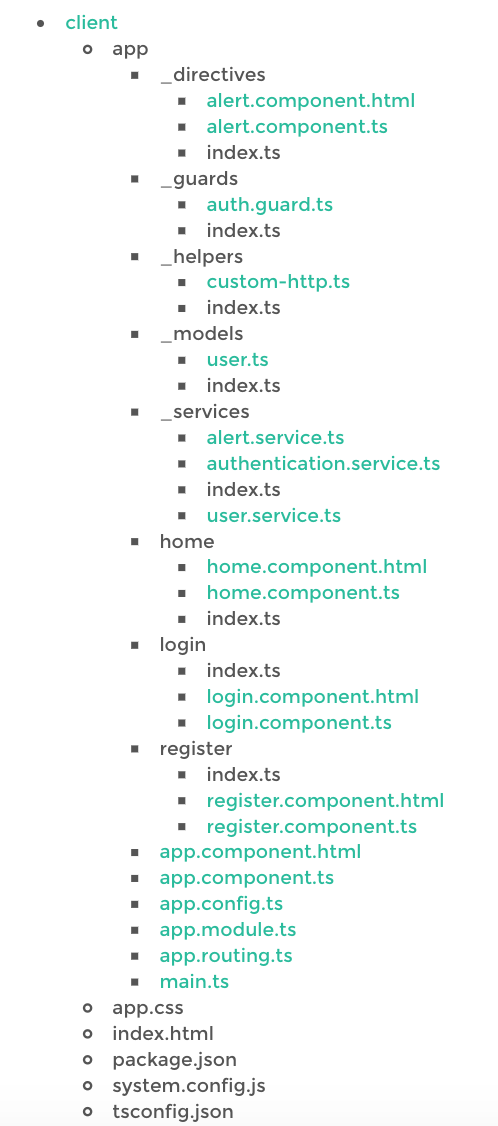
\includegraphics[width=30mm]{memoria/LaTeX/img/aplicacion/cliente.png}
    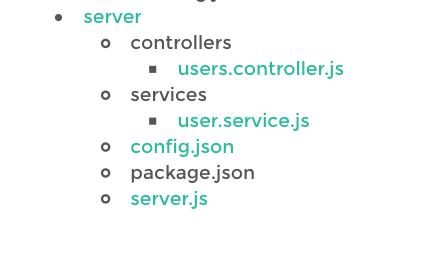
\includegraphics[width=30mm]{memoria/LaTeX/img/aplicacion/server.png}
    \caption[Estructura proyecto MEAN]{Estructura proyecto MEAN}
\end{figure}


\section{Node}

De los 4 grandes bloques he decidido empezar con Node, ya que es imprescindible para poder construir el proyecto.

Como ya he comentado en el capitulo anterior, Node es es un sistema innovador, puesto que es la plataforma encargada del funcionamiento del servidor, y funciona totalmente con JavaScript, como bien es sabido Javascript es un lenguaje de programación que en un principio era dedicado a correr en los navegadores, o en el lado del cliente, pero como se puede ver con el MEAN stack y sus subsistemas el uso de JavaScript se ha ampliado considerablemente a todos los aspectos de una página web.

Cabe destacar, sin duda, la irrupción en los últimos años de servidores interactivos asíncronos, como es el caso de NodeJS. Este tipo de servidores realizan tareas de forma asíncrona bloqueante, por lo que el tiempo de respuesta es, en muchos casos, menor que en servidores multihilos(servidores concurrentes). Por estos motivos, en la actualidad, múltiples proyectos enfocados al tiempo real, utilizan este tipo de servidores asíncronos.

De la mano a Node tenemos NPM, es el manejador de paquetes por defecto para Node.js. Para poder arrancar cualquier proyecto en MEAN, debemos utilizar npm para bajarnos todas las dependencias del proyecto. 

Una vez tengamos Node y NPM instalados, lo utilizaremos en los siguientes casos:

\begin{itemize}

\item \textbf{Instalar dependencias(Cliente y Servidor)}

\begin{lstlisting}
    sudo npm install
\end{lstlisting}

\item \textbf{Correr nuestro servidor}
\begin{lstlisting}
    sudo node server.js
\end{lstlisting}
    
\item \textbf{Arrancar el cliente: } 
\begin{lstlisting}
    sudo npm start
\end{lstlisting}
    
\end{itemize}

\section{Back-End: Express & MongoDB}
Nuestro lado servidor se compone de dos tecnologías muy importantes e innovadoras en el mercado de las aplicaciones web como son: Express, que como ya hemos comentado antes es un framework de desarrollo de aplicaciones web para Node.js y MongoDB que consiste en una base de datos NoSQL,el cual utiliza la librería mongoose para poder conectar node.js con la base de datos en MongoDB.

Comenzaré explicando el backend con el primer fichero que ejecutamos cuando queremos arrancar nuestro servidor Server.js

\subsection{Server.js} Para poder empezar analizando el código implementado en nuestro server.js, tenemos que saber como arrancar nuestro servidor.

\begin{lstlisting}
    sudo node server.js
\end{lstlisting}
    
Gracias a Node, simplemente con una linea en la terminal seremos capaces de generar procesos que escuchen en el puerto que queramos.

A continuación vamos a enumerar todas las funciones contenidas en nuestra server.js

\begin{enumerate}
    \item \textbf{Open mongo} Llamamos a la librería mongoogse encargada de unir a MongoDB con Node.js, a continuación le decimos a que data base apuntar y si el resultado es satisfactorio abrirá la conexión en caso contrario saltará la excepción.
\begin{lstlisting}
var mongoose = require('mongoose');
mongoose.connect('mongodb://localhost/classcity');
var db = mongoose.connection;
db.on('error', console.error.bind(console, 'conection error:'));
db.once('open', function() {
  console.log('Connected to Database');
});
\end{lstlisting}
    \item \textbf{Parser body} Analizamos los body de las request en un middleware antes que llegue a sus manejadores. 
\begin{lstlisting}    
app.use(bodyParser.urlencoded({ extended: true }));
app.use(bodyParser.json());
\end{lstlisting}
    \item \textbf{control errores} En caso de tener algún error en alguna solicitud, el manejador de errores se lanzará sin bloquear el resto del servicio.
\begin{lstlisting}    
app.use(function(err, req, res, next) {
  if (err.name === 'StatusError') {
    res.send(err.status, err.message);
  } else {
    next(err);
  }
});
\end{lstlisting}
    \item \textbf{control imágenes} Para poder controlar la ingesta de imágenes en nuestras bases de datos, hemos usado Multer, un middleware de node.js para el manejo multipart/form-data, que se usa principalmente para cargar archivos. 
    \begin{lstlisting}
var storage = multer.diskStorage({
    destination: function (req, file, cb) {
        cb(null, './uploads')
    },
    filename: function (req, file, cb) {
        console.log(file.fieldname);
        var name = file.fieldname + '-' + Date.now() + '.jpg';
        cb(null, name)
    }
})
var upload = multer({ storage: storage });
app.use(multer(upload).single('file'));
    \end{lstlisting}
    \item \textbf{Server sockets} Corremos nuestro chat en el puerto 8080, independientemente de nuestra aplicación que corre en el puerto 8000
    
\begin{lstlisting}
var socketServer = require('./controllers/socket');
socketServer.start();
\end{lstlisting}

    \item \textbf{Rutas} Nuestra aplicación se compone de multitud de rutas que invocan a funciones contenidas en nuestro controlador que mas tarde explicaremos.
\begin{lstlisting}
//Rutas
app.use('/', users);
app.use("/uploads",express.static(__dirname + '/uploads'), img);
img.route('/:id').get(Ctrlprofesor.getimg)
users.route('/loginalumno').post(Ctrlalumno.loginalumno);
\end{lstlisting}
    \item \textbf{Start server} Arrancamos nuestra aplicación en el puerto 8000
\begin{lstlisting}
app.listen(8080,'0.0.0.0', function() {
  console.log("Node server running on http://localhost:8080");
});
\end{lstlisting}
\end{enumerate}

\subsection{Estructura de la base de datos} 
Como bien sabemos MongoDB es una base datos no relacional, es decir no es como las típicas bases de datos SQL donde existen relaciones entre una tabla y otra. 

La estructura de la base de datos que he elaborado consiste en 4 modelos, los cuales se relacionan dos a dos por medio de referencias y el metodo populate en MongoDB.

Analizamos la estructura de los modelos:

\begin{itemize}
\item \textbf{Modelo Alumnos} Consiste en un modelo simple donde tenemos tres campos predefinidos de tipo string.
\begin{lstlisting}
var alumnoSchema  = new Schema({
  nombre:       { type: String },
  apellidos:    { type: String },
  edad:         { type: String }
});
module.exports = mongoose.model('Alumno', alumnoSchema);
\end{lstlisting}
\item \textbf{Modelo Login Alumnos} Este modelo encapsula dentro de él al anterior, y lo hace a partir de una llamada de referencia. Dentro del campo data tendremos el modelo del alumno.
\begin{lstlisting}
var loginSchema  = new Schema({
  email:         { type: String },
  password:     { type: String },
  data:    { type: Schema.ObjectId, ref: "Alumno"},
});
module.exports = mongoose.model('LoginAlumno', loginSchema);
\end{lstlisting}
\item \textbf{Modelo Profesores} Este modelo corresponde al del profesor.
\begin{lstlisting}
var profesorSchema  = new Schema({
  nombre:       { type: String },
  apellidos:    { type: String },
  edad:         { type: String },
  curso:        { type: String, enum:
    ['Primaria', 'ESO', 'Bachillerato', 'Universidad', 'FP',
    'EXAMENES LIBRES', 'FRACASO ESCOLAR'] },
  asignaturas:  { type: String},
  location: {
    type:       { type: String},
    coordinates: {type: []}
  },
  path:         {type: String},
  notification: {
    type: [{
      alumno: { type: Schema.ObjectId, ref: "Alumno"},
      leido: {type: Boolean},
      _id: false
    }]
  }
});
\end{lstlisting}
\item \textbf{Modelo Login Profesores} Modelo que vuelve a anidar otro modelo en el campo data.

\begin{lstlisting}
var loginSchema  = new Schema({
  email:         { type: String },
  password:     { type: String },
  data:    { type: Schema.ObjectId, ref: "Profesor"},
});
module.exports = mongoose.model('LoginProfesor', loginSchema);
\end{lstlisting}
\end{itemize}
La idea de tener estos modelos relacionados, es porque puede no interesarnos enviar toda la información en una llamada, es decir si un usuario hace introduce su email y su password en la ventana de login, no necesitaríamos buscar entre todos los datos de los usuarios, simplemente con tener un modelo con el login y la password de los usuario para poder hacer la verificación sería más que correcto.

\subsection{Controladores} Un controlador es un archivo donde tenemos diversas funciones que son invocadas a partir de la rutas que tenemos configuradas en el server.js. Dependiendo del modelo de la base de datos que utilicemos para guardar, editar o eliminar datos, he decidido organizar las funciones en tres controladores diferentes:

\begin{itemize}
\item \textbf{Controllers Alumnos} Es el fichero en el que están todas las funciones que usan los modelos alumno.js y loginalumno.js
\begin{enumerate}
    \item \textbf {registeralumno: } Función cuyo comportamiento consiste en comprobar que el email que introduce el alumno al registrarse no esta en nuestra base de datos, y que los campos password y email no están vacíos, en tales casos el servidor devolverá un 400 al cliente. 
    
    Si el alumno es registrado con éxito, se guardará en la base de datos y se enviarán las credenciales con un 201 en forma de token para una mayor seguridad.
    
    \begin{lstlisting}
alumno.save(function(err, datasave) {
  if(err) return res.send(500, err.message);
  var profile = _.pick(req.body, 'Email', 'Password','extra');
  profile.id = datasave.data;
  res.status(201).send({ id_token: createToken(profile) });
});
    \end{lstlisting}
    
    \item \textbf {loginalumno: } Si el alumno ya ha sido registrado en nuestra base de datos, y lo que quiero en hacer loguin, esta función sera invocada y comprobará que el email y la password del alumno coinciden con los credenciales, en caso de ser aceptado se le enviará sus credenciales en forma de token con un 201 y en caso de ser rechazado se le enviara un 400 con el mensaje: "The username or password don't match".
    
\end{enumerate}
\item \textbf{Controllers Profesores}Es el fichero en el que estan todas las funciones que usan los modelos profesor.js y loginprofesor.js
\begin{enumerate}
    \item \textbf {registerprofesor: }El comportamiento es idéntico a registeralumnos, con la única salvedad de que el modelo que utilizamos es profesor.js
    \item \textbf {loginprofesor: } También mismo comportamiento que en loginalumnos, pero utilizando el modelo de datos de loginprofesor.js
    
    \item \textbf {savenotificacion: } Cuando un alumno quiere contactar con un profesor vía chat, antes tiene que enviarle una petición de contacto. De esto consiste savenotification, es una función que se encarga de almacenar en la base de datos del profesor los alumnos que le han enviado una petición de contacto.
\begin{lstlisting}
exports.savenotificacion = function(req, res){
    DataProfesor.findOneAndUpdate(
        {_id: req.body._id},
        {$addToSet: {notification: {alumno: req.body.id, leido: false, _id: false}}},
        {safe: true},
        function(err, model) {
            if (err == null){
                res.status(200).send("La notificacion ha sido recibida");
            }else{
              res.send(500, err.message);
            }
        }
    );
};

\end{lstlisting}  
    
    \item \textbf {readynotificacion: }Es una función que se encarga de comprobar si el profesor a aceptado o rechazado la solicitud de contacto del alumno. En caso de ser aceptado, el chat se habilitará y el alumno y el profesor podrán tener un primer contacto.
    
    \item \textbf {getallprofesores: } Función que se encarga de enviar al cliente todos y cada uno de los profesores que integran Classcity sin ningún tipo de requisito. 
    \item \textbf {getimg: } Como podemos ver en el código, es una función muy simple que se encarga de enviar al cliente la imagen que solicita.
    \begin{lstlisting}
exports.getimg = function(req, res){
    res.sendfile('uploads/'+ req.params.id)
};
    \end{lstlisting}
    \item \textbf {postimg: } Función que se encarga de actualizar las imágenes de los profesores que editan su perfil. 
\begin{lstlisting}
exports.postimg = function(req, res){
  ProfesorScheme.findOne({"email" : req.file.originalname}, function(err, data) {
    DataProfesor.findById(data.data, function(err, dataext) {
        dataext.path = req.file.path;
        dataext.save();
    });
  });
  res.end('File is uploaded');
};
\end{lstlisting}
    
    \item \textbf {queryprofesores: } Continuamos con la función mas compleja de todas. Su misión consiste en filtrar los profesores que encajen con la solicitud, es decir como he comentado al principio, un alumno puede buscar a su profesor por tres argumentos diferentes: Curso, Asignatura y Distancia. 
    
    Por este motivo si nos fijamos en la función, hacemos un find con tres argumentos de entre los que destaca el argumento Location. La magia de mongoDB nos permite hacer query tan impresionantes como esta, donde tenemos una base de datos de ubicaciones de profesores más la ubicación que introduce el alumno somos capaces de devolverle aquellos profesores que se encuentren a un radio de él.

\begin{lstlisting}
exports.queryprofesores = function(req, res) {
  DataProfesor.find({"curso" : req.body.Curso, "asignaturas": req.body.Clase,
  location:{$geoWithin:{$centerSphere: [ [ req.body.Loc.lat, req.body.Loc.lng],
  req.body.Radio / 6378100 ] } } },  function(err, dataprof){
	      res.status(200).jsonp(dataprof);
  });
};
\end{lstlisting}
    
    \item \textbf {getdetail: } Por último concluimos con la función que se encarga de encontrar el perfil del profesor que el alumno solicita. 

\begin{lstlisting}
exports.getdetail = function(req, res){
  DataProfesor.findOne({"_id" : req.params.id}, function(err, dataprof) {
    res.status(200).send(dataprof);
  });
};

\end{lstlisting}
    
    
\end{enumerate}
\item \textbf{Controllers Socket} Socket.js es el fichero que se encarga de gestionar el chat en la parte del servidor. Si comenzamos analizando el código de socket.js, lo primero que hacemos es que el servidor escuche en el puerto 8000.
\begin{lstlisting}
server.listen(8000,'0.0.0.0');
\end{lstlisting}

Una vez que el servidor esta escuchando en el puerto 8000, debemos utilizar la librería io para establecer la conexión con el usuario que intenta tener la comunicación.

\begin{lstlisting}
io.on('connection', function(socket) {}
\end{lstlisting}

Como tenemos que manejar tantos hilos de chat como profesores tengamos, necesitamos un control de canales. Por eso cada 'room' nueva viene asociado con el identificador de cada profesor, es decir cuando un profesor se registra, un nuevo canal es creado y los alumnos tienes la oportunidad de poder hablar con el profesor en esa room sin que otros profesores se tengan constancia de ello.

Las 'room' son cada uno de los canales abiertos en la comunicación del chat, donde los alumnos son libres de elegir a que 'room' entrar. Cada vez que un alumno entra en el perfil de un profesor, entra en una 'room' donde solo los que estén en el perfil del profesor podrán enterarse de lo que se comente por esa 'room'.

\begin{lstlisting}
 socket.on('room', function(_room) {
    room = _room.roomName;
	user = _room.userName;
    socket.join(room);
    if (room in rooms)
        rooms[room]++;
    else
        rooms[room] = 1;
    io.to(room).emit('intro', {'userName': user, 'text': "ha entrado en la sala"});
});

\end{lstlisting}

Cuando un alumno o un profesor que ya se encuentran en una 'room' concreta empiezan a enviarse mensajes, la forma que tenemos para gestionarlo es la siguiente:

\begin{enumerate}
    \item El mensaje enviado por el emisor es recibido por el servidor
    
    \item El servidor analiza el mensaje enviado por el emisor y lo trata reconociendo a que 'room' pertenece.
    
    \item El servidor reenvía el mensaje a todo el mundo que se encuentre en esa 'room', excluyendo al emisor.
\end{enumerate}

\begin{lstlisting}
socket.on('newMessage', function(_room) {
			 user = _room.userName;
			 text = _room.text;
			 io.to(room).emit('message', {'userName': user, 'text': text});
			});
\end{lstlisting}

En caso de que alguno de los integrantes de la 'room' decida abandonar el chat, realizaremos los siguientes pasos:

\begin{enumerate}
    \item Recibiremos el disconnect del usuario que abandono la conexion.
    
    \item A continuación informaremos al resto de los integrantes de la 'room' que usuario en concreto abandono la sala.
    
    \item Y en el caso de que todos los integrantes incluyendo el profesor no se encuentren en la sala, la eliminaremos de nuestros datos de control.
    
\end{enumerate}

\begin{lstlisting}
socket.on('disconnect', function() {
    leaveRoom();
});

var leaveRoom = function() {
    rooms[room]--;
    io.to(room).emit('client left', {'userName': user, 'text': "dejo la sala"});
    if (rooms[room] === 0)
        delete rooms[room];
};
\end{lstlisting}


\end{itemize}

\section{Front-End: Angular}

De los 8 bloques principales de una app en Angular, vamos a ir identificando uno a uno y que uso se le da en nuestra aplicación.

\begin{figure}[H]
    \centering
    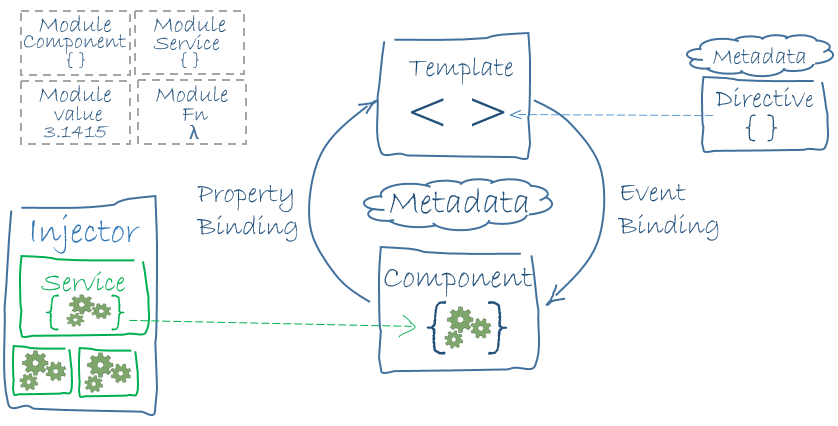
\includegraphics[width=110mm]{memoria/LaTeX/img/infraestructura/angular2Architecture.png}
\end{figure}

\subsection{Modulos: } Como ya sabemos las aplicaciones en Angular son modulares y un modulo es el conjunto de código dedicado a cumplir un único objetivo, en esta sección vamos a hablar de los modulos utilizados en nuestra aplicación.
\begin{itemize}
\item \textbf{NgModule from '@angular/core'} Es el modulo principal, el cual recibe un objeto que define el módulo. Los metadatos más importantes de un NgModule son:

\begin{enumerate}
\item{Declarations: } Las vistas que pertenecen a tu módulo. Hay 3 tipos de clases de tipo vista: componentes, directivas y pipes.
\item{Exports: } Conjunto de declaraciones que deben ser accesibles para templates de componentes de otros módulos.

\item{Imports: } Otros NgModules, cuyas clases exportadas son requeridas por templates de componentes de este módulo.

\item{Providers: } Los servicios que necesita este módulo, y que estarán disponibles para toda la aplicación.

\item{Bootstrap: }: Define la vista raíz. Utilizado solo por el root module.
\end{enumerate}

\item \textbf{RouterModule from '@angular/router'} es uno de los módulos más importantes de Angular, se encuentra dentro de la librería @angular/route, gracias a el cada vez que cambiemos de direccion URL cambiaremos de página sin necesidad de tener que interactuar con el servidor.

\item \textbf{ HttpModule, Http, RequestOptions from '@angular/http'} Otro modulo imprescindible en una aplicación Angular, se encuentra dentro de la librería @angular/http. Gracias a este módulo podemos hacer cualquier petición AJAX sin apenas tener que escribir código. 

\item \textbf{ FormsModule from '@angular/forms'} Modulo encargado de añadir formularios personalizados.

\item \textbf{FileUploadModule from 'ng2-file-upload'} Es el modulo que nos permite subir imágenes y enviarlas a nuestro servidor, para luego poder almacenarlas de forma ordenada en nuestra base de datos.

\item \textbf{AgmCoreModule from 'angular2-google-maps/core} Gracias a este modulo, podemos utilizar la API de google maps en nuestra aplicación.

\item \textbf{ BrowserModule from '@angular/platform-browser'} este modulo es necesario en cualquier app que se renderice en el navegador.


\item \textbf{ AuthGuard from './common/auth.guard'} Gracias a este modulo, podemos conservar las credenciales de un usuario durante un tiempo determinado en el navegador.

\item \textbf{ ProvideAuth, AuthHttp, AuthConfig from 'angular2-jwt'} Este modulo proporciona seguridad a nuestra aplicación, generando un token encriptado para cada usuario que se registre en nuestra aplicación.

\item \textbf{AppComponent, Intro, LoginAlumno, LoginProfesor , HomeAlumno, HomeProfesor, SignupAlumno, SignupProfesor, ProfesorDetail } Estos son los módulos propios que desarrollamos para nuestra aplicación, cada uno con su función independiente que contaremos a continuación.

\subsection{Componentes: }

Continuamos con los componentes de nuestra aplicación, como ya sabemos los componentes son como etiquetas nuevas, que podemos inventarnos para realizar las funciones que sean necesarias para nuestro negocio. 

Nuestra aplicación se compone de 1 componente principal y 8 componentes que derivan de él. AppComponent es el componente principal y tiene la siguiente apariencia:

\subsubsection{AppsComponent }
\begin{lstlisting}
import { Component } from '@angular/core';

@Component({
  selector: 'app-root',
  templateUrl: './app.component.html',
  styleUrls: ['./app.component.css']
})
export class AppComponent {
  title = 'ClassCity';
}
\end{lstlisting}

El selector app-root o el nombre de la etiqueta que se usará cuando se desee representar, con la propiedad templateUrl asociamos un archivo .html que se usará como vista del componente. Por último se define su estilo mediante la propiedad StyleUrls, indicando a un array de todas las hojas de estilos que deseamos.

\subsubsection{Componentes secundarios }

\begin{itemize}
\item \textbf{Intro} Este componente corresponde con la pagina introductoria a la aplicación donde podemos elegir entre que perfil de usuario queremos adoptar: Profesor o Alumno.

\item \textbf{LoginAlumno, LoginProfesor} Componentes encargados de realizar la función de loguin del alumno o del profesor. Hemos desarrollado una función que se encarga de realizar una petición POST al servidor, si la respuesta es aceptada se almacenarán las credenciales en el "localstorage" con un timeout de 1 hora. Mientras que si la petición es rechazada, el servidor nos enviará un mensaje avisando de que: "The username or password don't match"

\item \textbf{SignupAlumno, SignupProfesor} Estos componentes se van a encargar de registrar a profesores y alumnos en nuestra base de datos, para ellos hemos desarrollado una función en cada componente, que simplemente se encarga de enviar al servidor una petición POST con un body donde se encuentran los datos personales del profesor o el alumno.

\item \textbf{HomeAlumno, HomeProfesor} Cuando un profesor o un alumno, es aceptado dentro de nuestra base de datos y consigue entrar en el home de la aplicación, puede realizar diferentes funciones dependiendo de si entro como alumno o como profesor. 

\begin{enumerate}
\item \textbf{Alumno }  Un alumno, puedo realizar la búsqueda del profesor que mas le interese por diferentes parámetros:
\begin{itemize}
    \item{El curso en el que esta el alumno}
    \item{La asignatura que quiere cursar}
    \item{La distancia a la que se encuentre el profesor}
\end{itemize}
    
\item \textbf{Profesor } El home del profesor consiste en un chat realizado con websocket, donde el profesor podrá entablar relación con cualquier alumno que este interesado en él. Aparte de poder personalizar su perfil, cambiando la foto que cada profesor tiene como avatar.
\end{enumerate}
\end{itemize}

\item \textbf{ProfesorDetail} Como último componente tenemos ProfesoDetail, cuando un alumno encuentra a su profesor particular ideal desde el home del alumno y hace click sobre él profesor interesado, el componente ProfesorDetail se lanza y consiste en una ficha técnica del profesor particular, así como un chat donde el alumno podrá comunicarse con el profesor para poder quedar y acordar el precio de la clase. 
 
\end{itemize}

\subsection{Templates: } Como bien sabemos, los templates son las plantillas que se utilizan para dar forma a las aplicaciones, es la parte más visual de una aplicación web y es la propia magia de Angular quien se encarga de renderizar estas plantillas, haciendo aplicaciones mucho mas personalizadas para el usuario. A continuación vamos a ir analizando una a una las diferentes templates que forman la aplicación:

\item \textbf{intro.html} Cuando accedemos a https://www.classcity.tk, la primera plantilla que se nos presenta es Intro.html. Según podemos ver en la imagen, consiste en una pagina introductoria donde podemos elegir si somos alumnos o porfesores.

\begin{figure}[H]
    \centering
    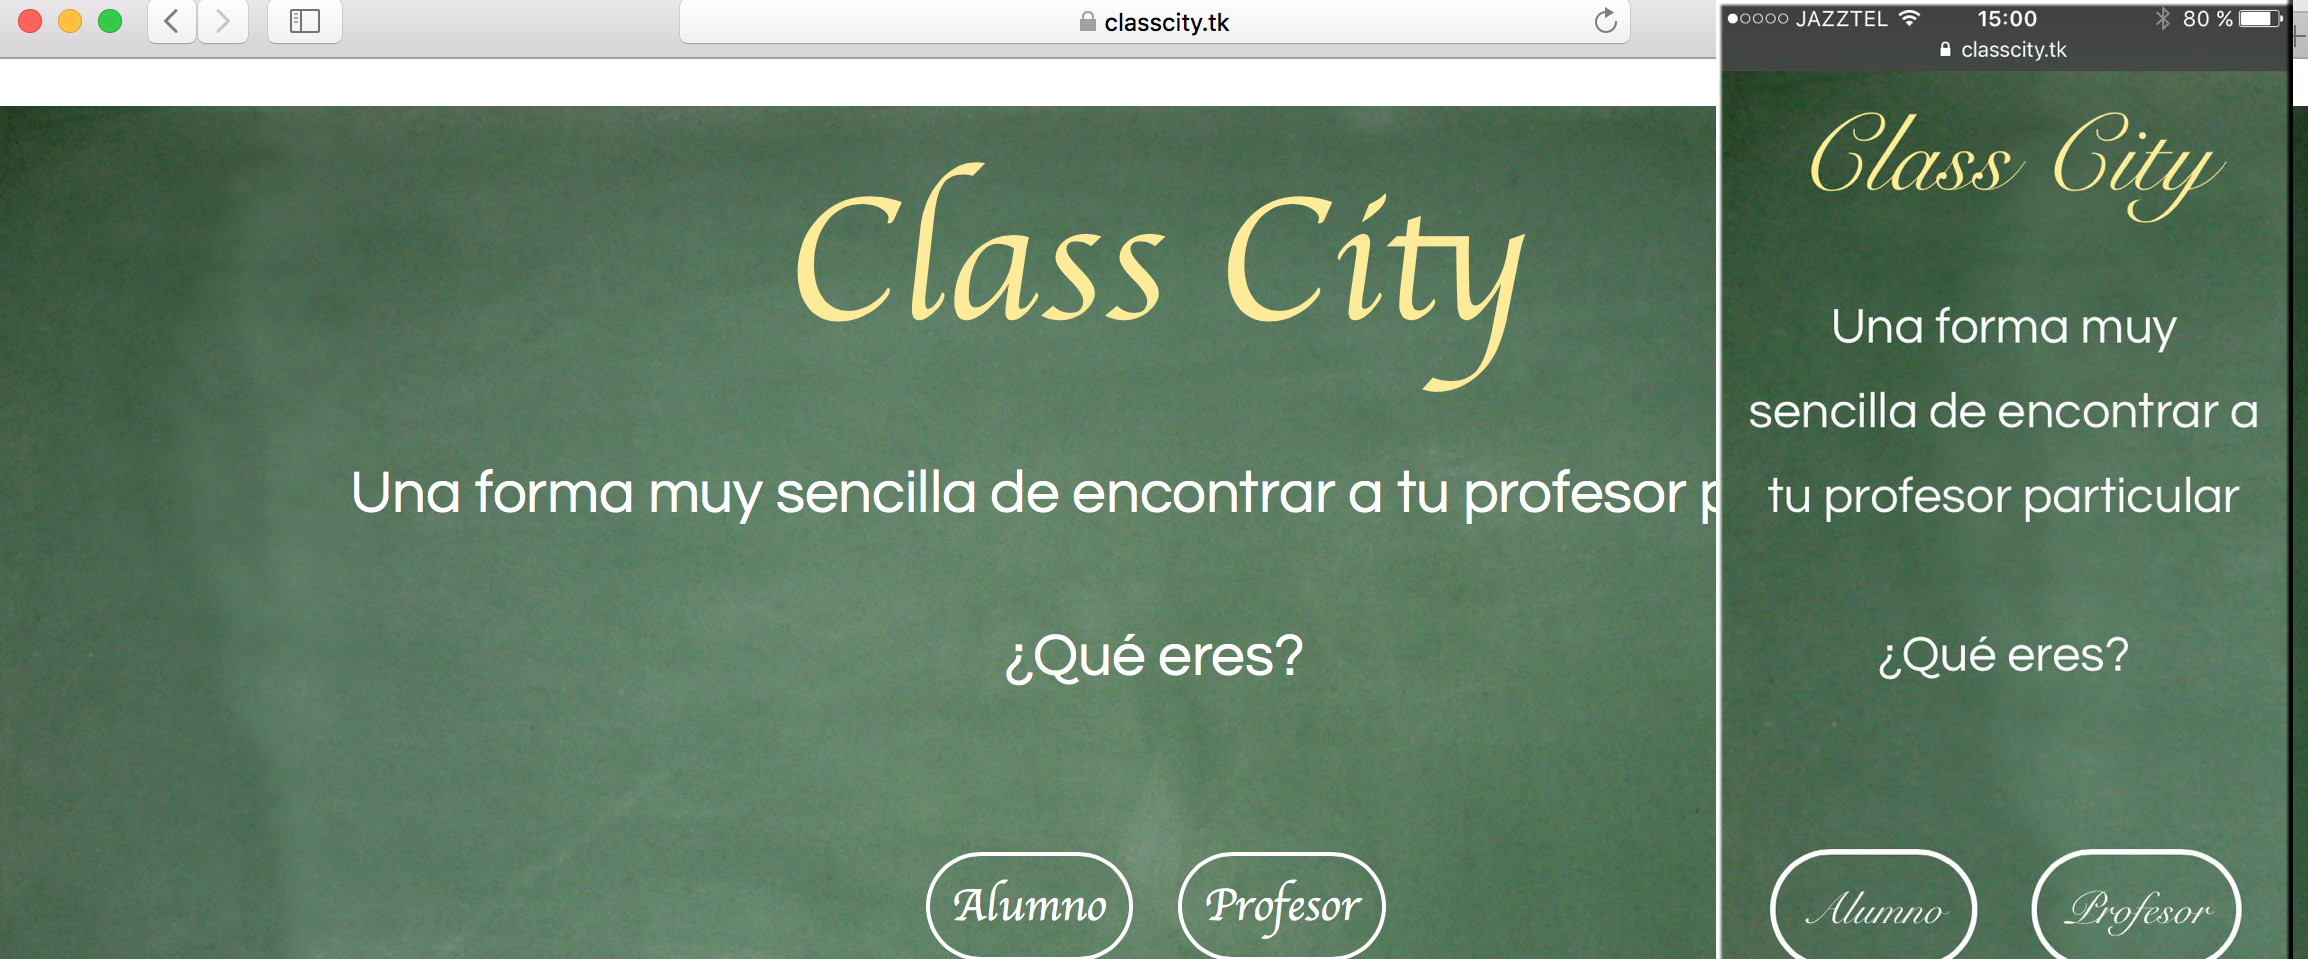
\includegraphics[width=110mm]{memoria/LaTeX/img/templates/intro.png}
\end{figure}

\item \textbf{loginalumno.html} Al seleccionar dentro de Intro.html en Alumno, accedemos a la siguiente plantilla donde podemos visualizar un formulario con sus campos username y password.

\begin{figure}[H]
    \centering
    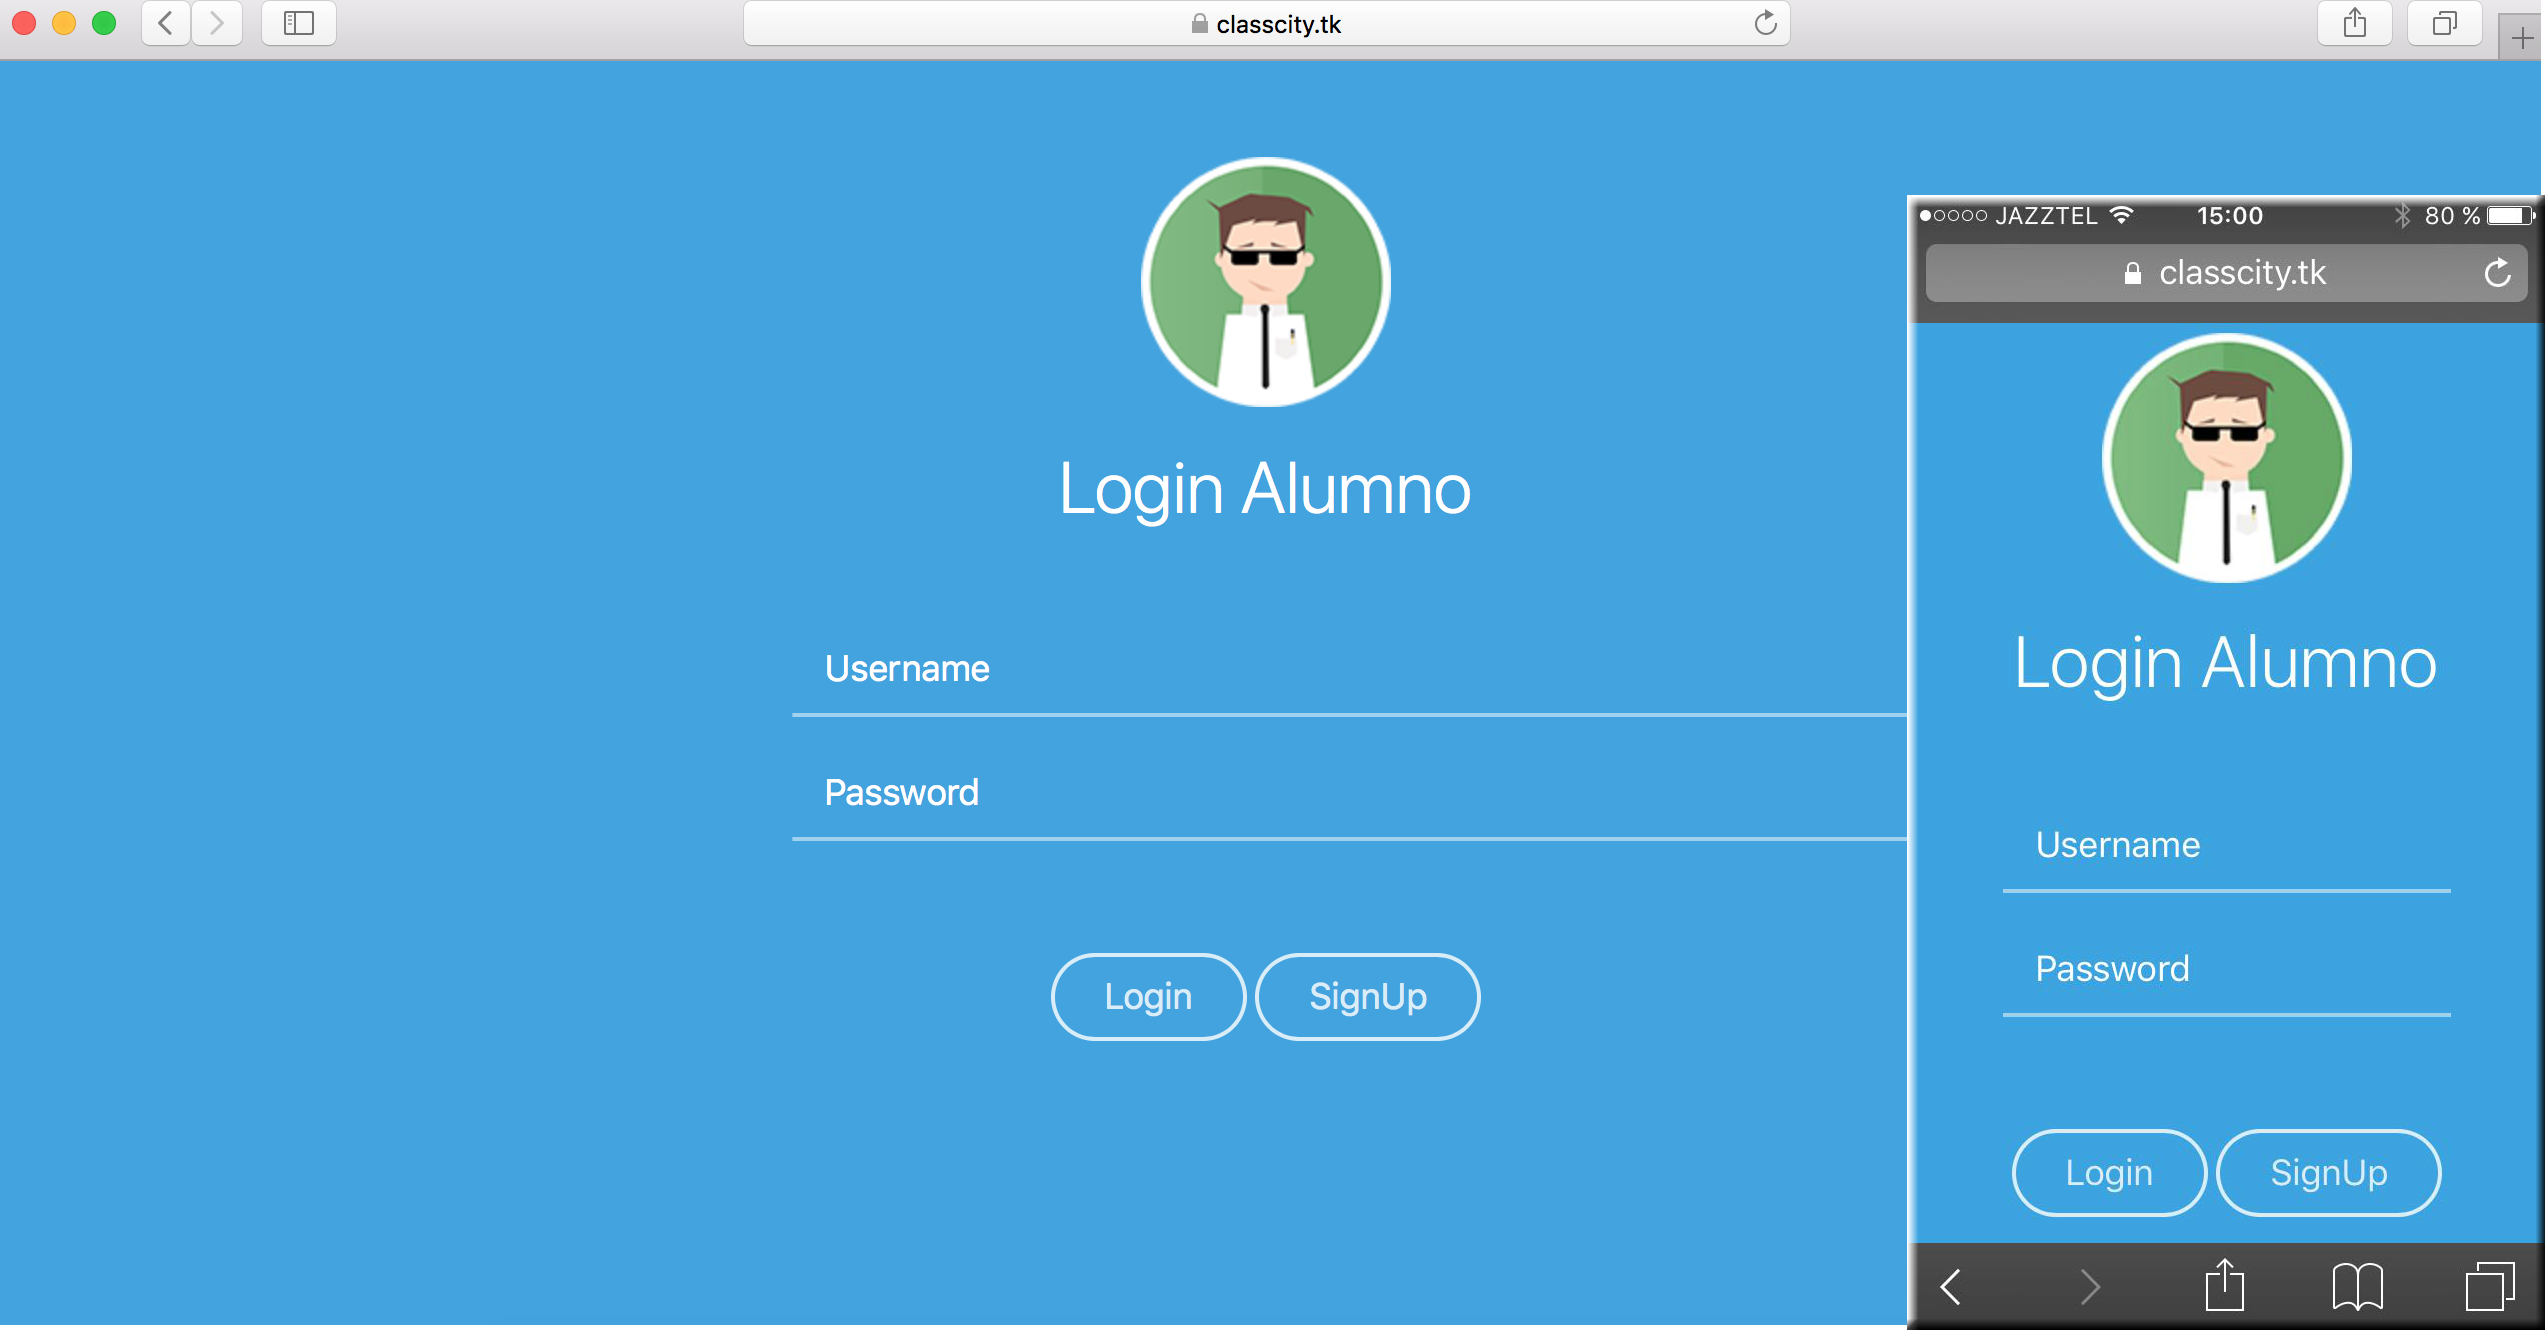
\includegraphics[width=110mm]{memoria/LaTeX/img/templates/loginalumno.png}
\end{figure}


\item \textbf{loginprofesor.html} Si en vez de seleccionar Alumno hubiesemos seleccionado Profesor, hubiesemos entrado en otro formulario donde los profesores ya registrados pueden acceder a la aplicación.

\begin{figure}[H]
    \centering
    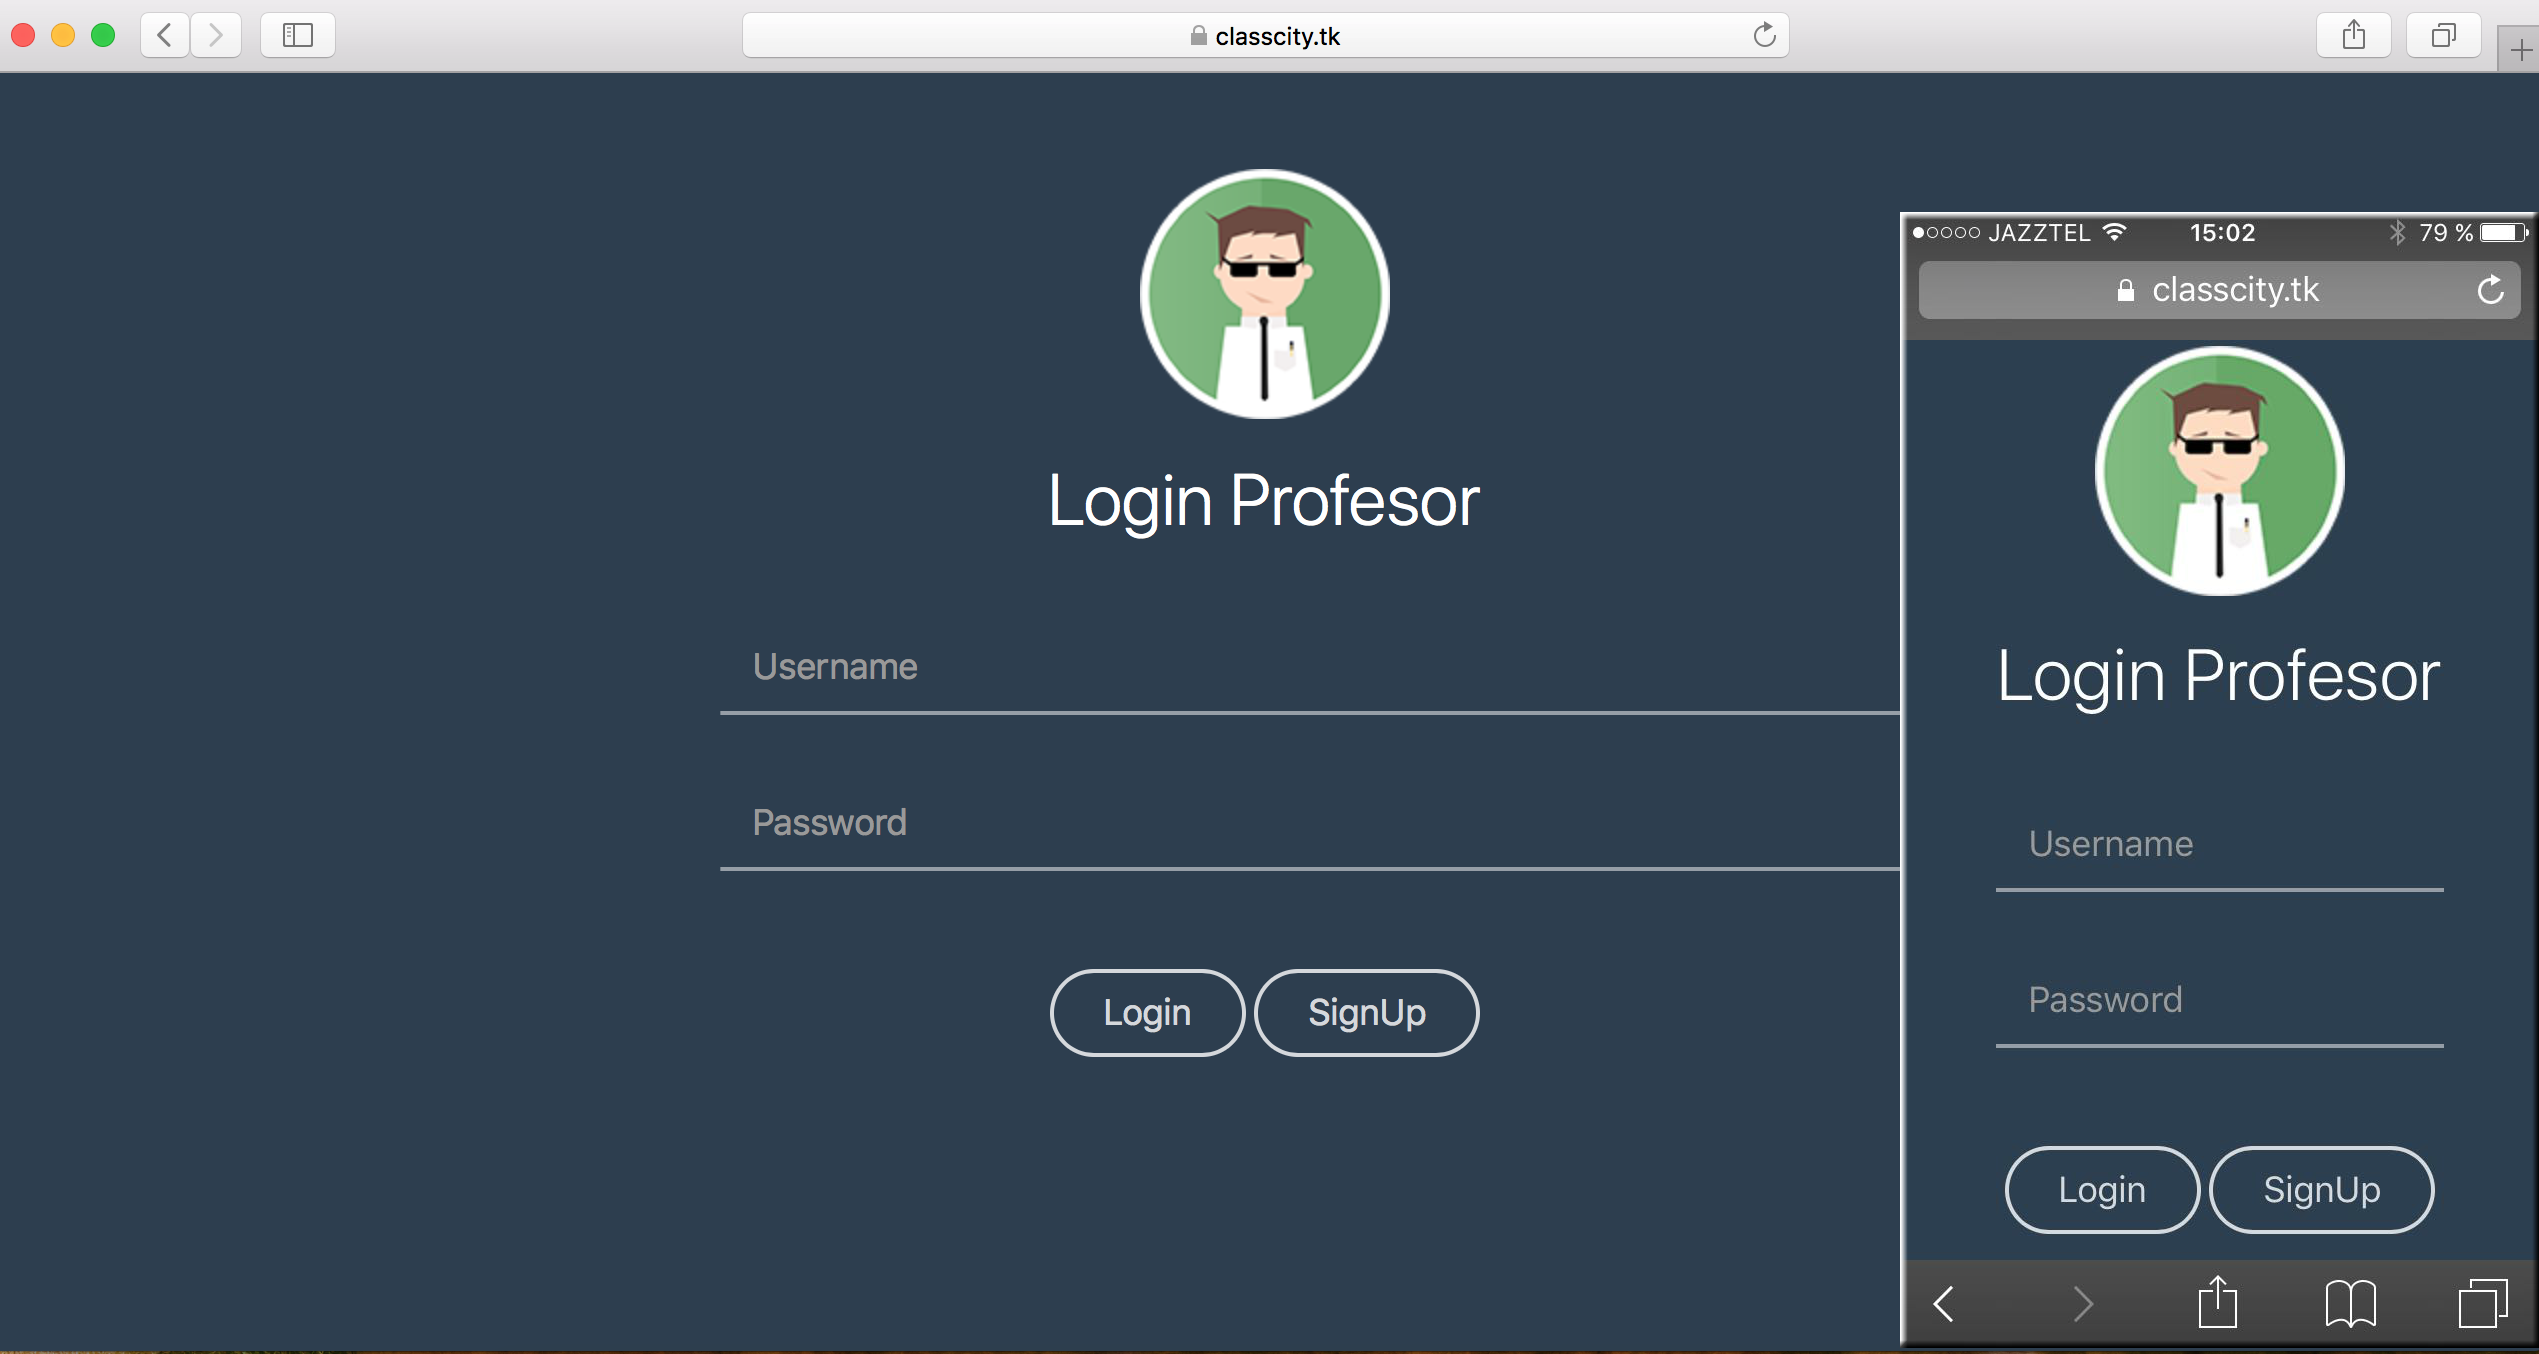
\includegraphics[width=110mm]{memoria/LaTeX/img/templates/loginprofesor.png}
\end{figure}

\item \textbf{registeralumno.html} Si un alumno quiere registrase simplemente debe entrar en SignUp, donde tendrá un formulario para poder completar todos los campos necesarios. 
\begin{figure}[H]
    \centering
    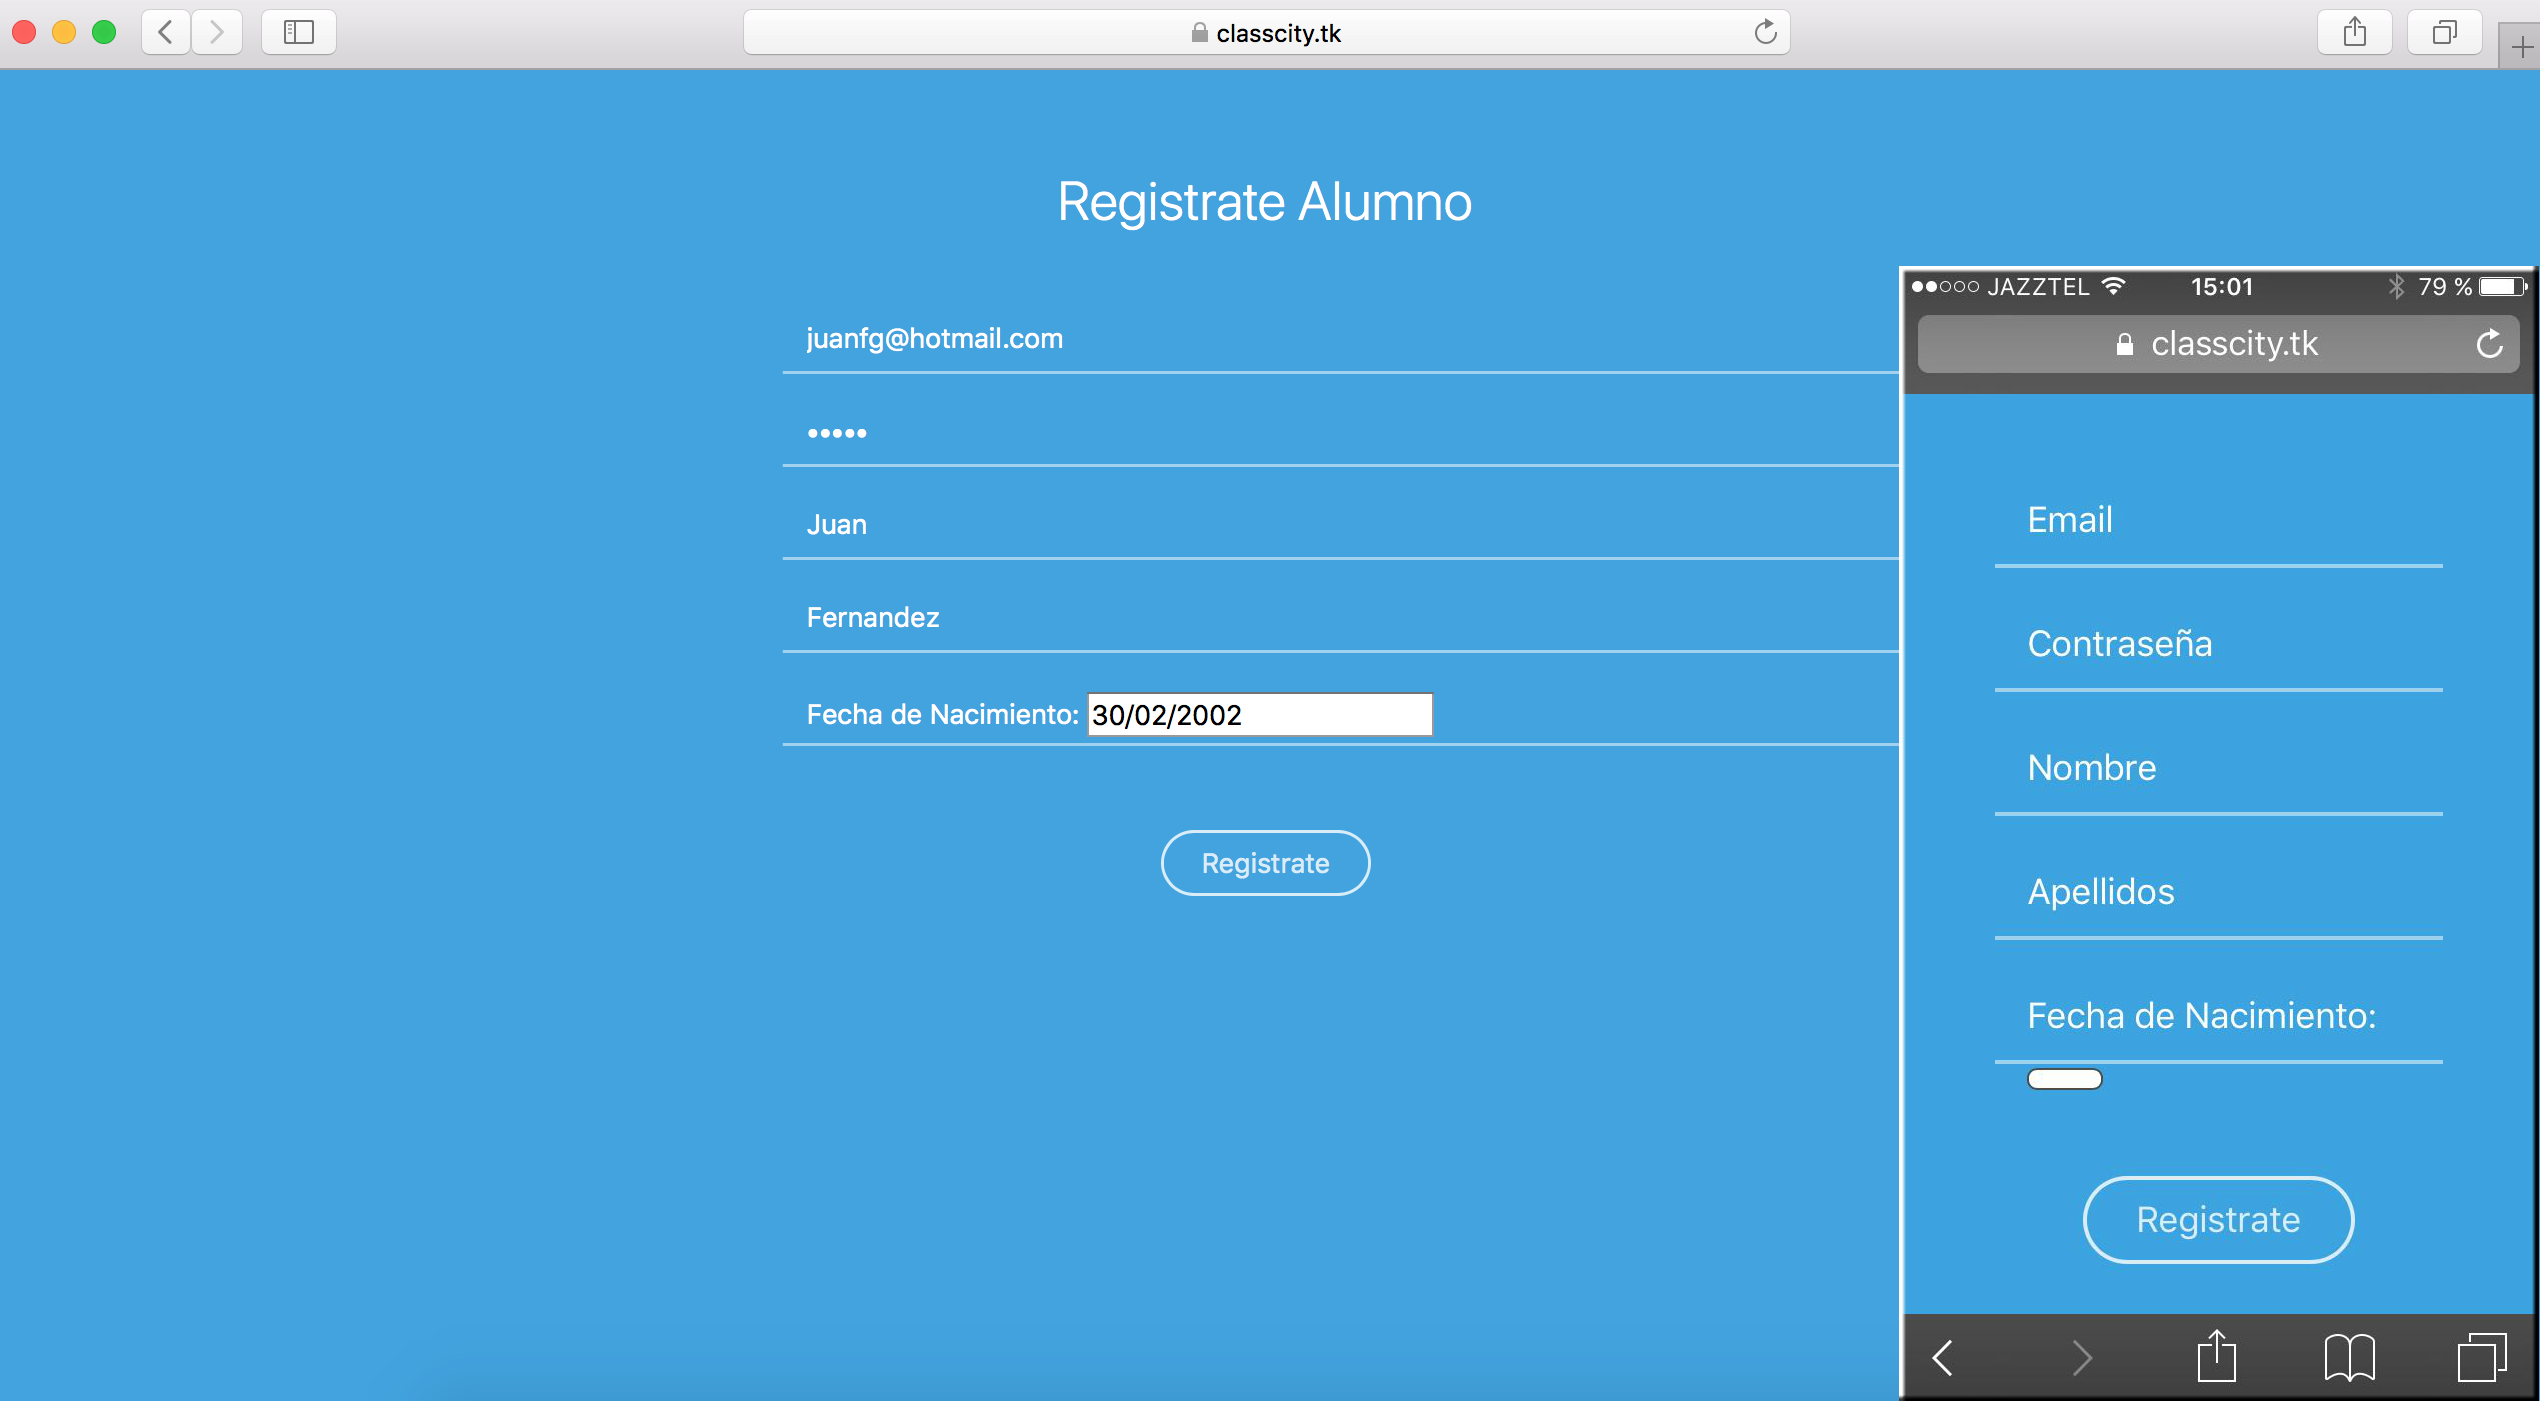
\includegraphics[width=110mm]{memoria/LaTeX/img/templates/registeralumno.png}
\end{figure}

\item \textbf{registerprofesor.html} Si es el profesor es quien quiere registrarse en nuestra aplicación, entrará en SignUP de profesores e introducirá los datos necesarios.
\begin{figure}[H]
    \centering
    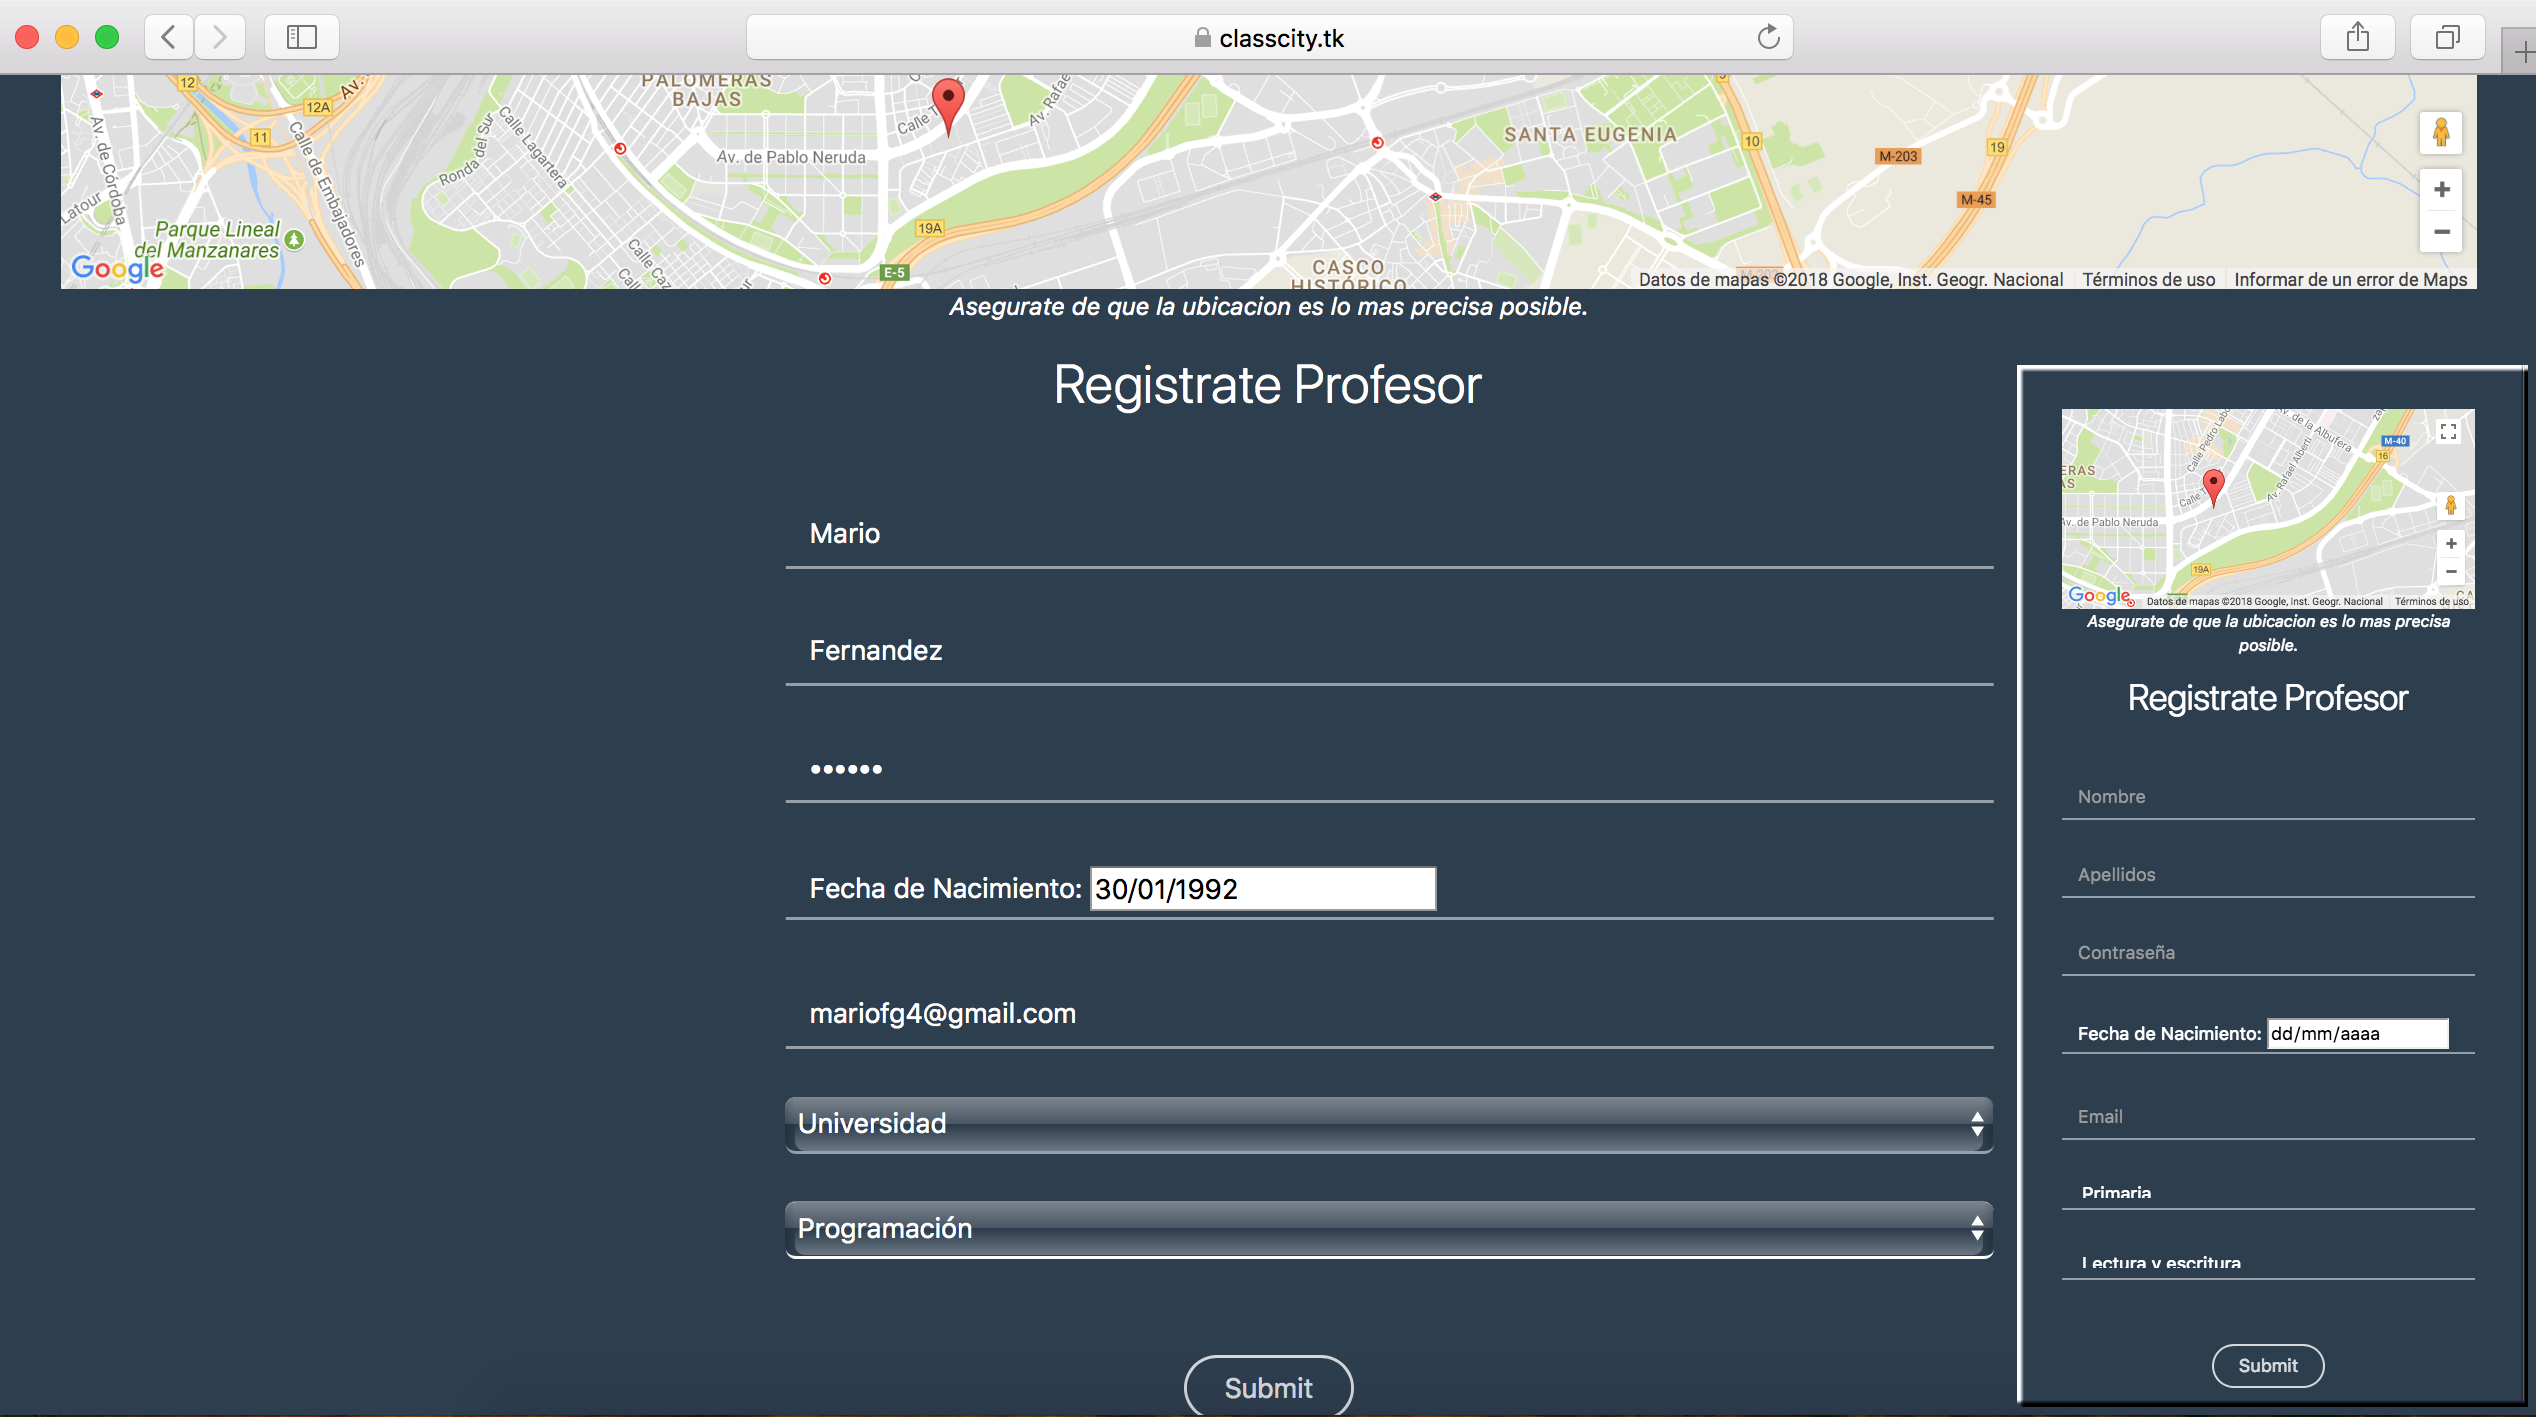
\includegraphics[width=110mm]{memoria/LaTeX/img/templates/registerprofesor.png}
\end{figure}

\item \textbf{homealumno.html} Una vez que el alumno ya ha sido registrado en nuestra base de datos, la interfaz con la que se encontrará el alumnos es la que podemos ver en la siguiente imagen. 
Donde podemos encontrarnos con un Input para introducir la ubicación donde queremos buscar, por defecto nos ubicará en Madrid, Centro. También podemos diferenciar los filtros de búsqueda que tenemos donde marcamos: El curso, La asignatura y la distancia máxima en la que queremos buscar a nuestro profesor. Por último cuando el alumno busca con los parámetros que desee, les aparecerá pintados en el mapa tantos profesores como haya en nuestra aplicación con esas especificaciones.
\begin{figure}[H]
    \centering
    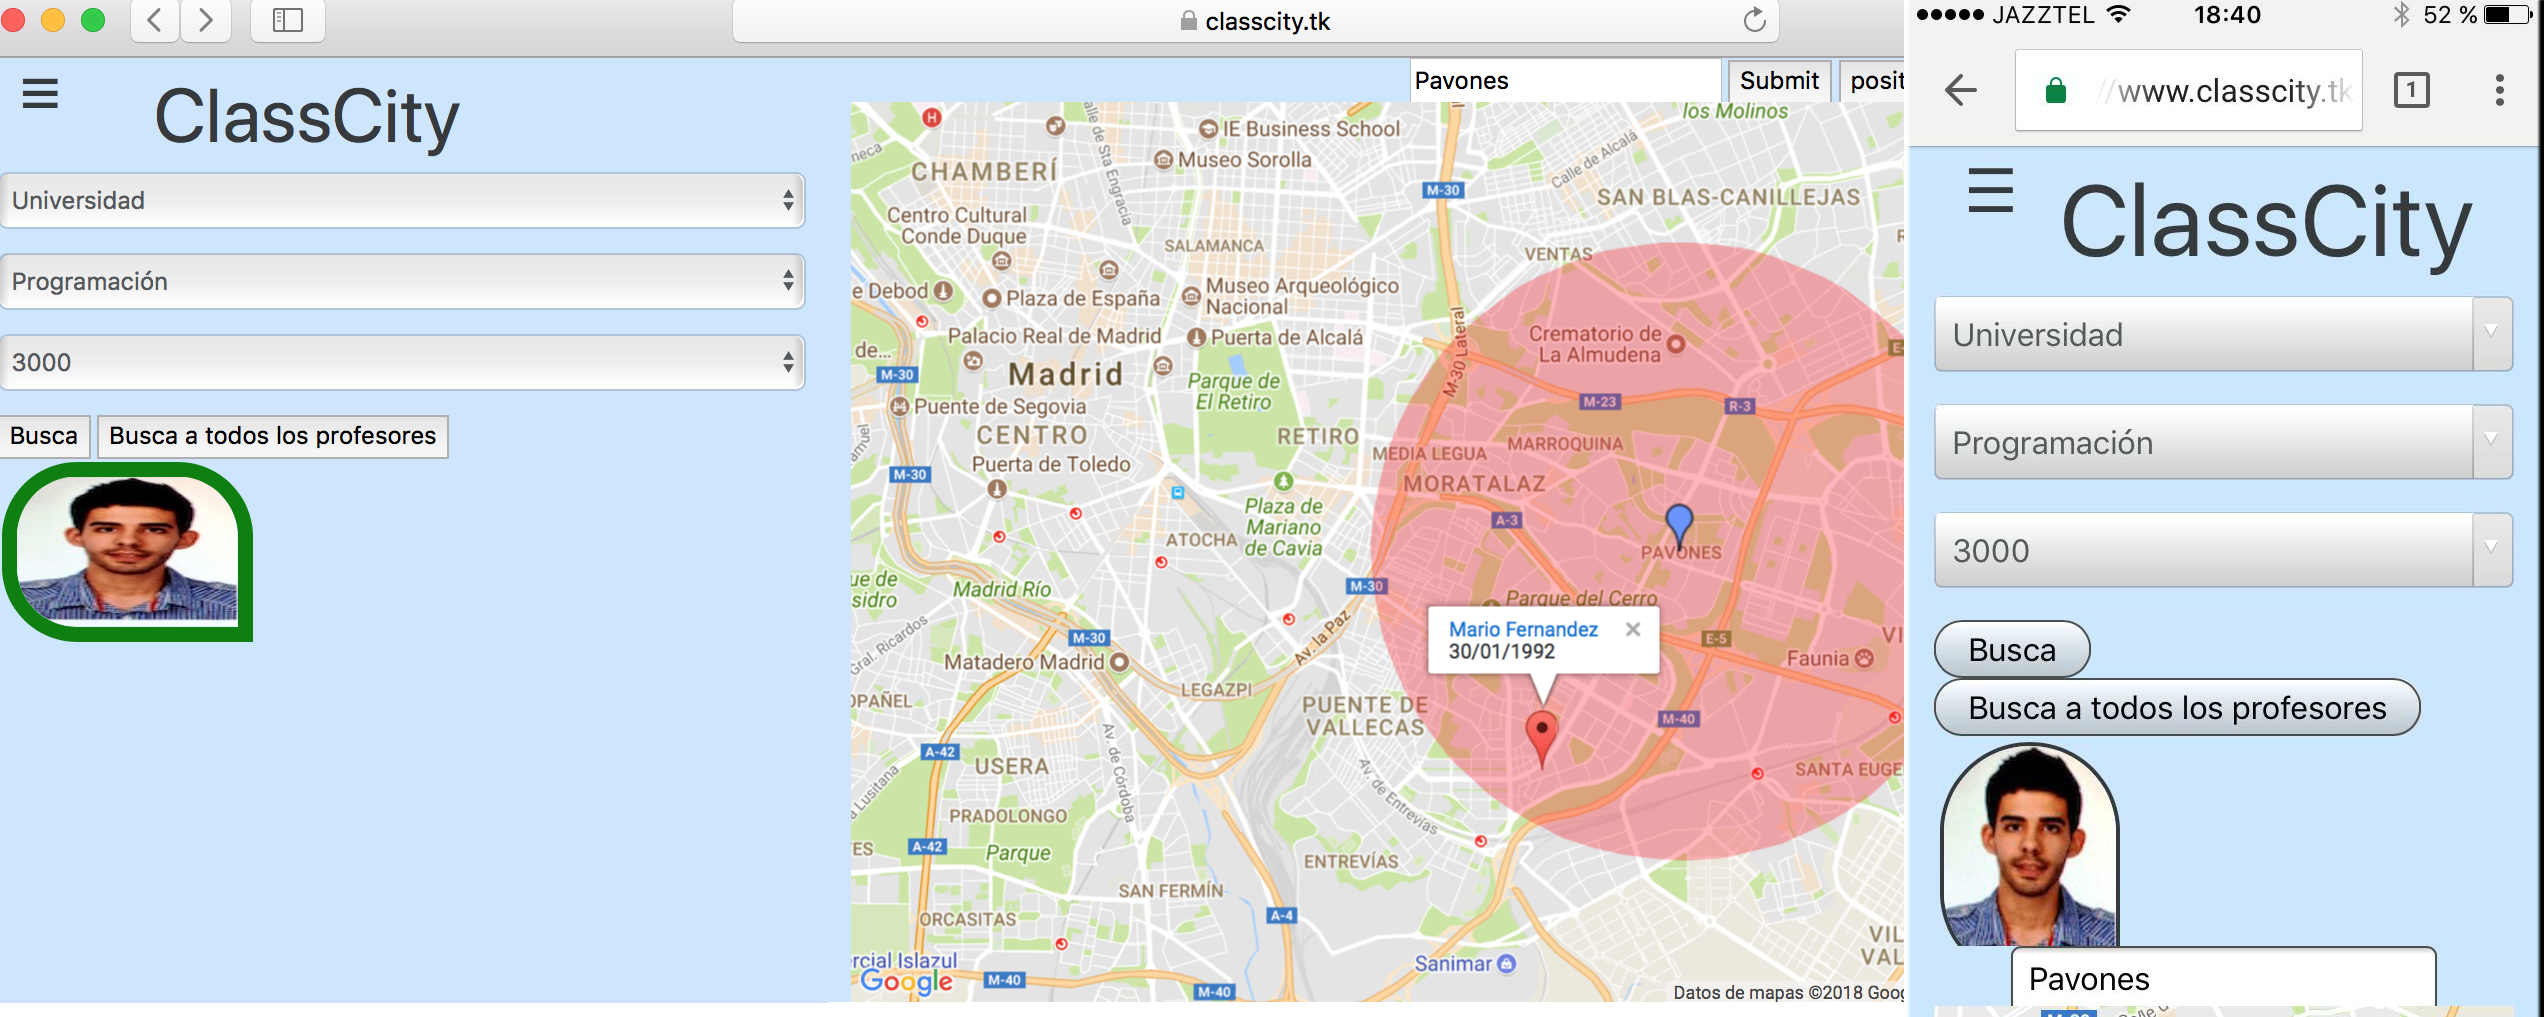
\includegraphics[width=110mm]{memoria/LaTeX/img/templates/homealumno.png}
\end{figure}

\item \textbf{detail.html} Cuando el alumno encuentra algún profesor de su interés, puede hacer click sobre la imagen del porfesor y así poder entrar en mas detalle, viendo su ficha técnica y pudiendo entablar una conversación a partir del chat.
\begin{figure}[H]
    \centering
    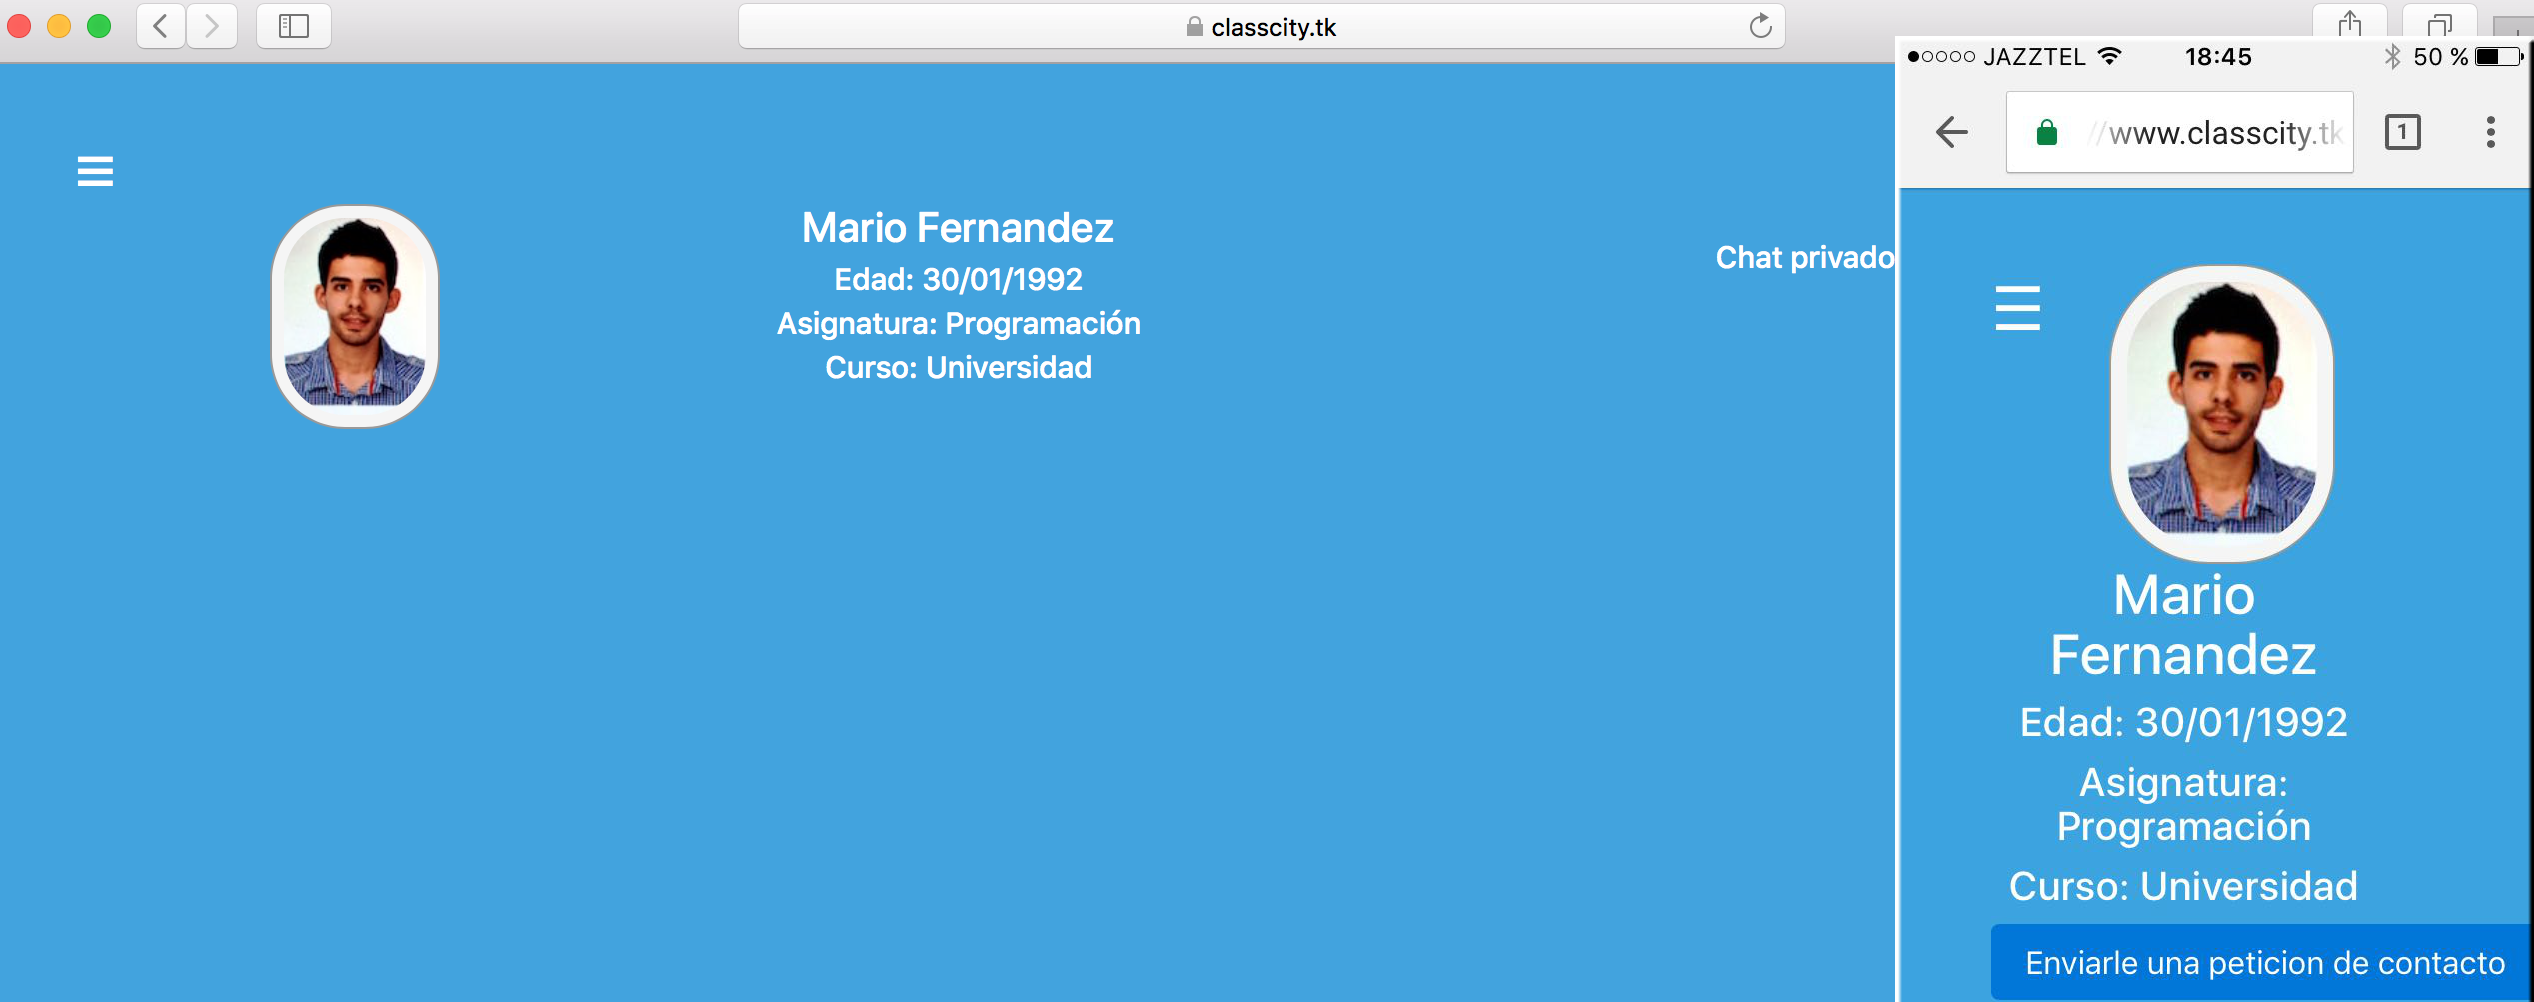
\includegraphics[width=110mm]{memoria/LaTeX/img/templates/detailprof.png}
\end{figure}

\item \textbf{homeprofesor.html} Cuando el profesor ya ha sido registrado en nuestra aplicación, el home del profesor es habilitado y en él puede hablar por un chat privado con todos los alumnos que le escriban por su canal, además de poder editar la foto de su perfil. 
\begin{figure}[H]
    \centering
    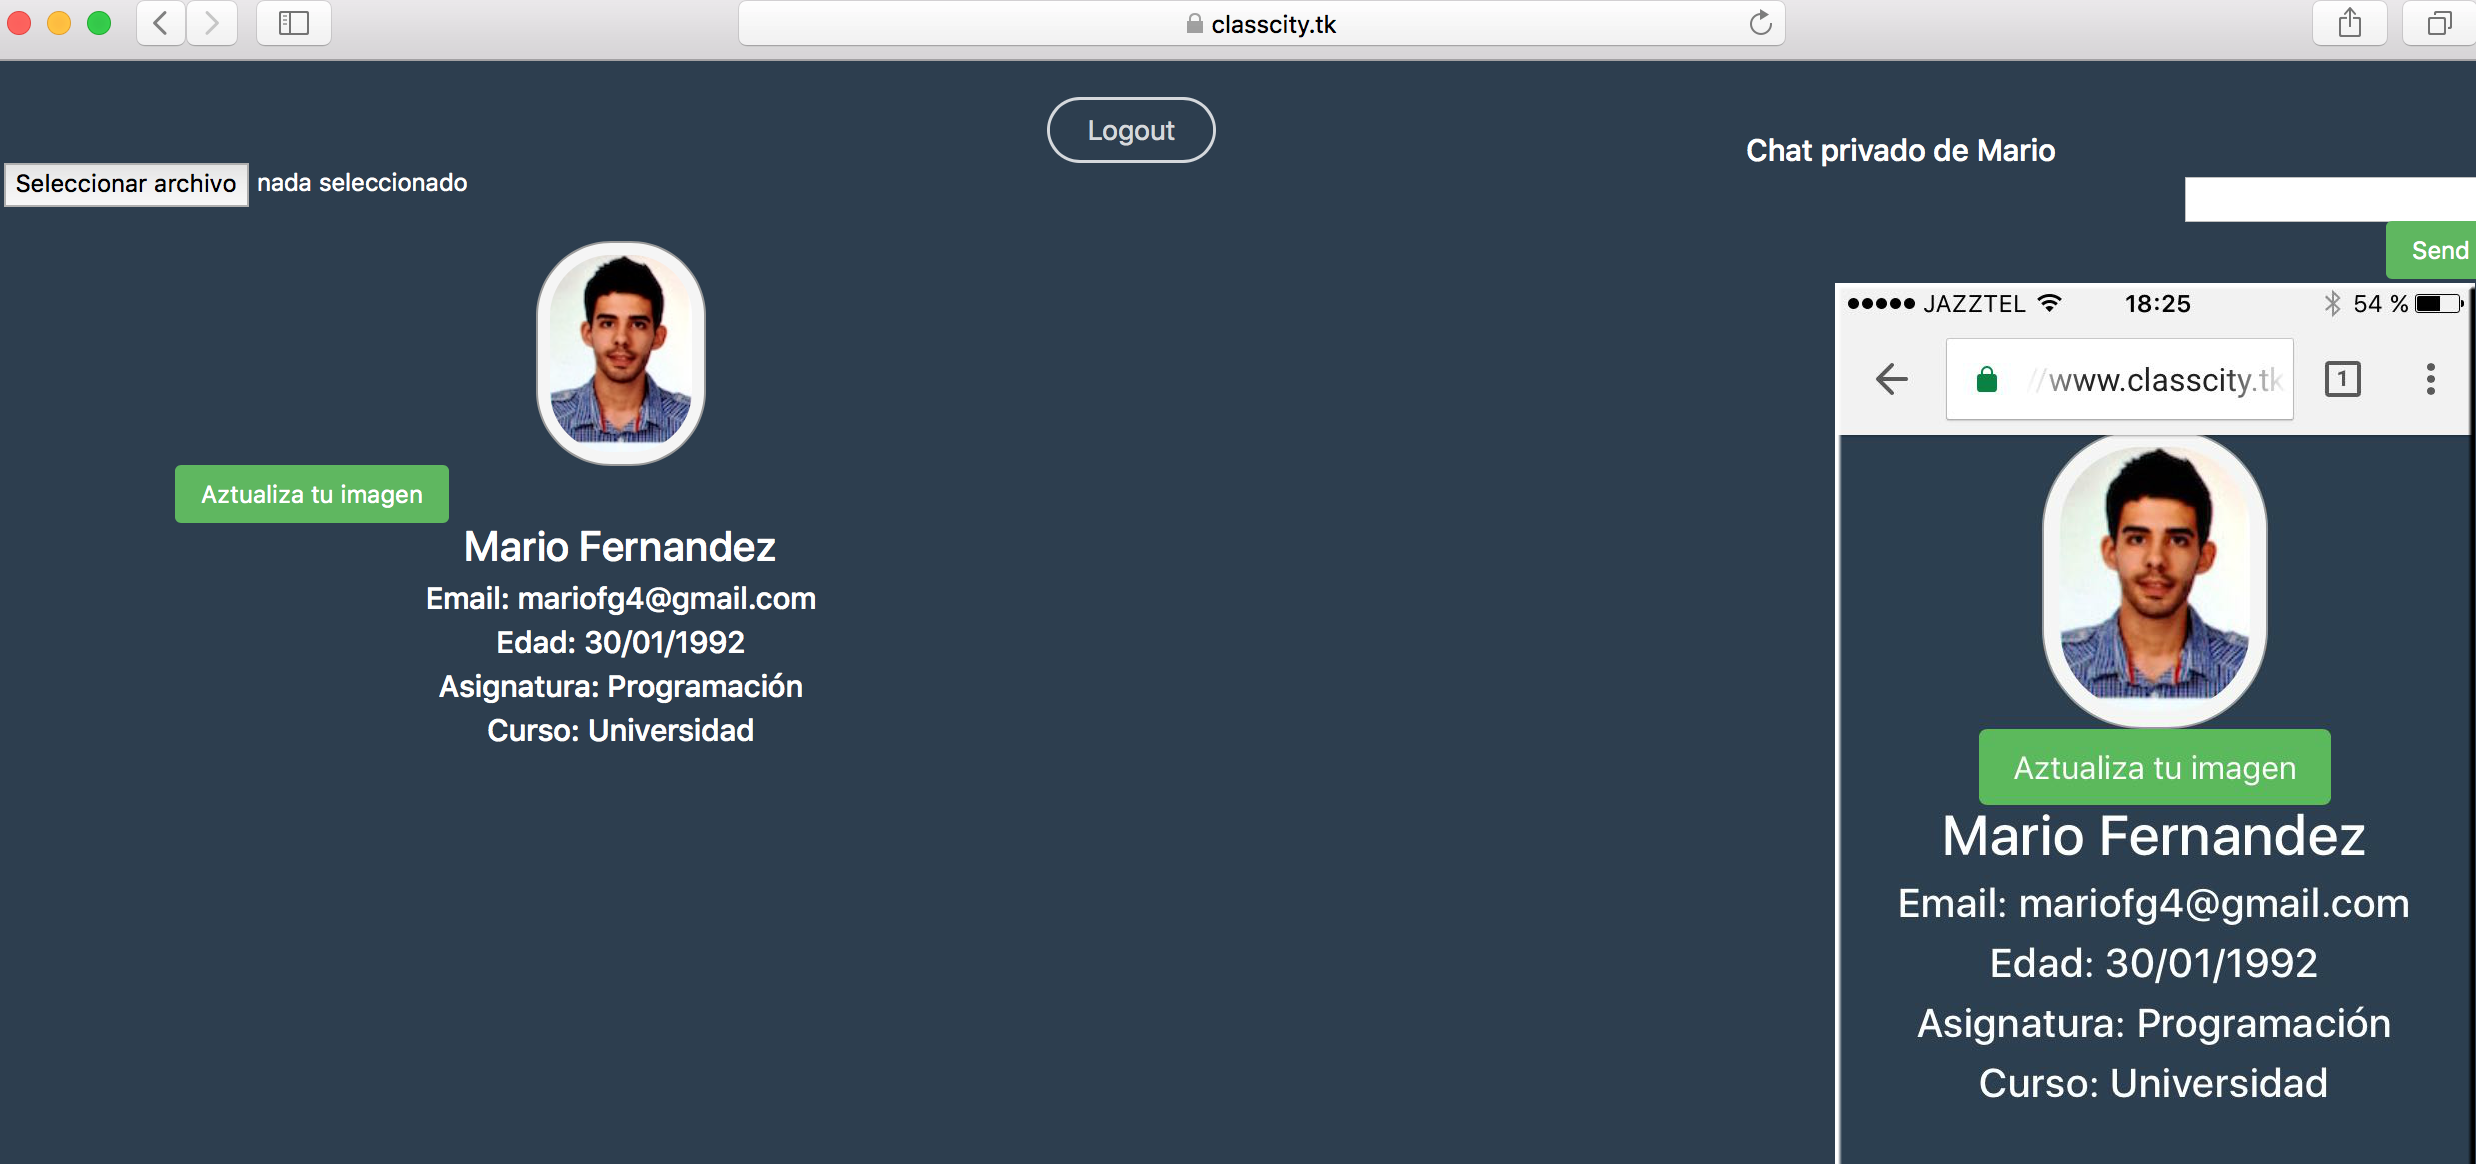
\includegraphics[width=110mm]{memoria/LaTeX/img/templates/homeprof.png}
\end{figure}

\subsection{Metadatos: }
\subsection{Data Binding: } El Data Binding nos abstrae de la lógica pull/push asociada a insertar y actualizar valores en el HTML y convertir las respuestas de usuario(inputs, clicks, etc) en acciones concretas.

Como he comentado en el tema anterior Angular tiene 4 formas de Data Binding, las cuales hemos utilizado en nuestra aplicación para realizar las siguientes funciones:

\item \textbf{Interpolación(Hacia el DOM)} Angular evaluá todas las variables e introduce su resultado en el DOM. En el siguiente caso estamos insertando en el arbol DOM, todos los datos del usuario, consiguiendo una apariencia de la pagina mucho mas personalizada.

\begin{lstlisting}
<code>{{decodedJwt.Email}}</code></pre>
<code>{{decodedJwt.id.nombre}}</code></pre>
<code>{{decodedJwt.id.apellidos}}</code></pre>
<code>{{decodedJwt.id.edad}}</code></pre>
\end{lstlisting}

\item \textbf{Property binding: (Hacia el DOM))} Este tipo de Data Binding, permite pasar los objetos que nosostros queramos de nuestro componente padre('home') a la propiedad (Latitud, Longitud, radius, fillColor) del componente hijo, en este caso sebm-google-map-circle. Para ello el componente hijo tiene que tener predefinido ciertas entradas en su directiva.

\begin{lstlisting}
<sebm-google-map-circle 
    [latitude]="query.Loc.lat" 
    [longitude]="query.Loc.lng"
    [radius]="query.Radio"
    [fillColor]="'red'">
</sebm-google-map-circle>
\end{lstlisting}

\item \textbf{Event binding: (Desde el DOM)}
Si queremos invocar a una función cuando se lance un evento, como por ejemplo cuando queremos hacer click en el boton de LogOut. En el momento que hacemos click sobre el boton de logout, la función logout es invocada y salimos de la sesión.

\begin{lstlisting}
<button type="Submit" (click)="logout()">Logout</button>
\end{lstlisting}

\item \textbf{Two-way binding: (Desde/Hacia el DOM)}

Cuando queremos combinar el Event Binding y el Property Binding tenemos el binding bi-direccional, como podemos ver en el siguiente ejemplo.

\begin{lstlisting}
<input [(ngModel)]="address">
\end{lstlisting}

En este caso queremos que el valor de address se actualice en el componente y que a su vez se introduzca dentro del input como en el caso de property binding.

\subsection{Directiva: }Como ya he comentado las directivas son como los componentes, pero sin un template asociado. En nuestro caso hemos utilizado directivas para realizar según que funciones, por ejemplo:

\item \textbf{FileSelectDirective, FileDropDirective, FileUploader} Estas tres directivas proceden del modulo "FileUploadModule", y sirven para poder subir una imagen desde tu escritorio local al navegador, para luego poder enviar la imagen al servidor destino.

\begin{lstlisting}
<input type="file" ng2FileSelect [uploader]="uploader" />
\end{lstlisting}
\item \textbf{sebm-google-map, sebm-google-map-marker} Estas son otras de las directivas procedentes del módulo "agmCoreModule", el cual nos proporciona toda la api de GoogleMaps. Gracias a estas directivas podemos jugar con el Api de google en nuestra aplicación angular.

\begin{lstlisting}
<sebm-google-map *ngIf="query.Loc"
    [latitude]="query.Loc.lat" 
    [longitude]="query.Loc.lng"
    [scrollwheel]="false" [zoom] = "13">
    <sebm-google-map-marker
        [latitude]="query.Loc.lat"
        [longitude]="query.Loc.lng"
        [iconUrl] = "iconUrl">
    </sebm-google-map-marker>
</sebm-google-map>
\end{lstlisting}

También tenemos que hablar de los otros dos tipos de directivas que hemos usado en nuestra aplicación.

\item \textbf{Directivas Estructurales: *ngFor} repite su elemento en el DOM una vez por cada item que hay en el iterador que se le pasa, siguiendo una sintaxis de ES6. 

\item \textbf{Directivas Atributo: ngModel} Implementa un mecanismo de binding bi-direccional. En este ejemplo el elemento HTML '<'select'>', asigna la propiedad value a mostrar y además responde a eventos de modificación.
\begin{lstlisting}
<div class="form-group">
    <select class="form-control" [(ngModel)]="query.Curso" name="curso">
        <option *ngFor="let p of curso" [value]="p">{{p}}</option>
    </select>
</div>
\end{lstlisting}

\subsection{Servicio: } Como ya sabemos los servicios se definen a través de simples clases y son imprescindibles en Angular, ya que toda función o valor es encapsulado dentro de un servicio.

\item \textbf{AlumnoService} Este servicio se encarga de convertir una dirección física a una coordenada(latitud, longitud) para poder representarlo en el mapa. 

Si observamos detenidamente el código, lo primero que hacemos en la función "getLatLan(address: string)" es una petición a la API de google maps con una dirección y esperamos a que nos responda. La respuesta puede ser satisfactoria o no, en caso de que sea OK las variables lat y lng serán actualizadas con los valores devueltos por google maps, si por el contrario no hubiesemos recibido respuesta, un mensaje de error sera mostrado por pantalla.
\begin{lstlisting}
export class AlumnoService {
  getLatLan(address: string) {
    let geocoder = new google.maps.Geocoder();
    return Observable.create(observer => {
      geocoder.geocode( { 'address': address}, function(results, status) {
        if (status === google.maps.GeocoderStatus.OK) {
          let obj: Object = {lat: results[0].geometry.location.lat(),
            lng: results[0].geometry.location.lng() };
            observer.next(obj);
            observer.complete();
        } else {
            console.log('Error - ', results, ' & Status - ', status);
            observer.next({});
            observer.complete();
        }
      });
    });
  }
}
\end{lstlisting}


